\documentclass[12pt]{article}

\usepackage{amssymb,amsmath}
\usepackage[margin=1.0in]{geometry}
\usepackage{fancyhdr} % required for custom header
\usepackage{graphicx}
\usepackage{listings}
\usepackage{courier}
\usepackage[usenames,dvipsnames]{color}
\usepackage[maxfloats=30]{morefloats}
\usepackage{caption}
\usepackage{subcaption}


%set up the header
\pagestyle{fancy}
\lhead{Trever Hines}
\chead{El Mayor Postseismic}
\rhead{\today}

\setlength{\headheight}{15pt}
\renewcommand\headrulewidth{1.0pt} % Size of the header rule

%% Title
%%------------------------------------------------------------------------------
\title{	
El Mayor Postseismic
\author{Trever Hines}
\rule{\headwidth}{1.0pt}
}

 
 
\begin{document}
\maketitle
\section*{Abstract}
we propose a anelastic phase of deformation in the mantle distinct from phases associated with attenuation

\section*{Introduction}

Previous studies which have modeled postseismic deformation following the El Mayor-Cucapah earthquake include \cite{Pollitz2012}, \cite{Gonzalez-ortega2014}, \cite{Spinler2015}, and \cite{Rollins2015}. \cite{Gonzalez-ortega2014} was able to describe five months of near field ($\lesssim 50$ km from the epicenter) postseismic defomation observed by InSAR and campaign GPS with afterslip and fault contraction on the coseismically ruptured fault. \cite{Gonzalez-ortega2014} also noted that their preferred model underestimated the GPS displacements for stations $\gtrsim 25$ km from the rupture and suggested that it could be the result of unmodeled viscoelastic relaxation.  Using continuous GPS stations within 200 km of the El Mayor-Cucapah epicent, which consists mostly of stations north of the US-Mexico border, \cite{Rollins2015} found that three years of postseismic deformation can be adequately explained by afterslip in an elastic lithosphere, albeit with an implausibly large amount of afterslip inferred on the least constrained southern most fault segment which may be acting as a proxy for distributed relaxation in the lower crust or upper mantle. In this paper, we reiterate this finding by \cite{Rollins2015} and note that a purely elastic dislocation model is incapable of describing deformation observed at GPS stations greater than ~200 km from the El Mayor-Cucapah epicenter.  

Given the inability to describe both near and far field deformation with fault slip in an elastic lithosphere, \cite{Pollitz2012}, \cite{Rollins2015} and \cite{Spinler2015} have explored viscoelastic relaxation in the lower crust and upper mantle as a potential deformation mechanism. The lithospheric rheology is largely unknown and so modeling postseismic deformation with viscoelastic relaxation requires one to assume a rheologic model and find the best fitting model parameters, which is generally a computationally expensive nonlinear inverse problem. Consequently, a simplified structure for the lithosphere must be made to minimize the number of rheologic parameters that need to be estimated.  For example, it is commonly assumed that the lithosphere consists of only three homogeneously Maxwell viscoelastic layers, which may be an inadequate representation of the lithosphere \cite{Hines2013}\cite{Riva2009}. Additionally, it is necessary to make simplifying assumptions about the nature of afterslip. For example, one can assume a frictional model for afterslip and parameterize afterslip in terms its the unkown rheologic properties (e.g. \cite{Johnson2009} \cite{Johnson2004}). Additionally, one can assume that afterslip only dominates the first year of deformation (e.g. \cite{Pollitz2012} and \cite{Spinler2015}) and that viscoelastic relaxation is the dominant mechanism in later years. However, numerous observations of interseismic fault creep has been recognized in this and similar tectonic settings and it has been speculated that such creep can be initiated as a postseismic process \cite{Cakir2012} \cite{Cetin2014}.  We are unaware of any oIn this study, we therefore do not make to implicit assumption that afterslip terminates after a given amount of time.  Indeed, the preferred viscoelastic model from \cite{Pollitz2012} underpredicts near field velocities, which could be indicative of unmodeled continued afterslip.

All of the aforementioned studies model displacements observered at stations within 200 km of the El Mayor-Cucapah epicenter, while postseismic deformation in this region following previous earthquakes of similar magnitude has been observed at distances extended out to about 300 km \cite{Freed2007a}. In the present study we examine stations within 400 km of the El Mayor-Cucapah epicenter, which turns out to be crucial for discerning the postseismic deformation mechanism.

Clearly, both afterslip and viscoelastic relaxation are involved in postseismic deformation neglecting to model one of these deformation mechanisms could result in a biased estimate of the other.  In this paper we use the inverse method described in \cite{Hines2015} to estimate the afterslip an effective viscosity necessary to describe the transience postseismic deformation over the first ten months after the El Mayor-Cucapah earthquake. We then form a suite of models which have various lithospheric rheologies but viscosities that are consistent with the effective viscosity estimated from the early postseismic deformation. Of the suite of models tested, we find that five years of postseismic deformation can be explained by a combination of sustained afterslip on the coseismicly ruptured fault and a Zener rheology upper mantle with viscosity that decays from $4\times10^{18}$ to $1\times10^{18}$ Pa s. 


\section*{Data Processing}

We use continuous GPS position time series provided by University Navstar Consortium (UNAVCO) for Plate Boundary Observatory (PBO) stations within a 400 km radius about the El Mayor-Cucapah epicenter. Our analysis is on the coseismic and postseismic deformation resulting from the EMC earthquake, which we collectively describe as $u(t)$. We consider GPS position time series, $u_\mathrm{obs}(t)$, to be the superposition of $u(t)$, secular tectonic deformation, annual and semi-annual fluctuations, and coseismic offsets from sigificant earthquakes over the time span of this study.  The June 14, 2010 Mw5.8 Ocotillo earthquake and the August 26, 2012 Brawley swarm, which consisted of a Mw5.5 and Mw5.3 event, are the only earthquakes after the EMC earthquake that produced noticeable offsets recorded by GPS. Although the Ocotillo earthquake had its own series of aftershocks (Haukson), neither earthquake produced transient deformation that is detectable with GPS. We thus model $u_\mathrm{obs}(t)$ as 

\begin{equation}
  u_\mathrm{obs}(t) = u_\mathrm{pred}(t) + \epsilon
\end{equation}
where
\begin{equation}\label{TimeSeriesModel}
  \begin{split}  
    u_\mathrm{pred}(t) = &u(t) + c_0 + c_1t + \\
                         &c_2\sin(2\pi t) + c_3\cos(2\pi t) + c_4\sin(4\pi t) + c_5\cos(4\pi t) + \\
                         &c_6H(t-t_\mathrm{oc}) + c_7H(t-t_\mathrm{bs}).
  \end{split}
\end{equation}
In the above equations, $t_\mathrm{oc}$ and $t_\mathrm{bs}$ are the times of the Ocotillo earthquake and Brawley swarm respectively, $H(t)$ is the Heaviside function, $c_0$ through $c_7$ are unknown coefficients, and $\epsilon$ is noise with zero mean and variance that assumed known.

Stations which recorded signals that clearly cannot be described by the aforementioned processes are not included in our analysis. This includes stations in the Los Angeles basin, which record deformation that is largely anthropogenic. In order to ensure an accurate estimation of the secular deformation, we only use stations that were installed at least six months prior to El Mayor-Cucapah earthquake. While several stations were installed after the EMC earthquake to improve the spatial resolution of postseismic deformation \cite{Spinler2015}, our inverse method uses postseismic displacements rather than velocities (e.g. ...)
ELABORATE ON VELOCITY VS DISPLACEMENT
, which requires the knowledge of the stations preseismic position. Despite our inability to utilize potentially rich data, we prefer to use postseismic displacements rather than potentially dubious estimates of postseismic velocities.

The October 16, 1999 Hector Mine earthquake, which occurred within our study region about 270 km north of the EMC epicenter, has produce transient postseismic deformation which we do not wish to model either mechanically or through empirical line fitting. We thus restrict our analysis to deformation observed six years after the Hector Mine earthquake, past which point postseismic deformation for nearfield sites occurs at an approximately steady rate \cite{Savage2009}. When considering stations further away from the Hector Mine epicenter, postseismic transience persists for only about two years \cite{Spinler2015}.

Studies of postseismic deformation typically assume a parametric form for $u(t)$ such as such as a logarithmic or exponential function. Such functions have been found empirically e.g. \cite{Savage2005a} and theoretically \cite{Marone1991} to adequately describe deformation resulting from postseismic deformation. However, by assuming a logarithmic or exponential form of $u(t)$ we run the risk of overfitting the GPS time series and inferring a nonexistent postseismic signal. We therefore do not assume any parameteric form for $u(t)$ and rather treat it as integrated Brownian motion, so that 
\begin{equation}
    \dot{u}(t) = \sigma^2\int_0^t w(s) ds.
\end{equation}    

where $w(t)$ is white noise and the variance of $\dot{u}(t)$ increases linearly with time by a factor of $\sigma^2$. We use a
Kalman filtering approach to estimate $u(t)$ and the unknown parameters in eq. \ref{TimeSeriesModel} which we describe now.  In the context of Kalman filtering, our time varying state vector is
\begin{equation}
    \mathbf{X}(t) = [u(t),\dot u(t), c_0, ..., c_7]
\end{equation}
and eq. \ref{TimeSeriesModel} is the observation function which maps the state vector to the GPS observations. We initiate the Kalman filter by assuming a prior estimate of $\mathbf{X}(t)$ at time $t_0$ which has a sufficiently large covariance to effectively make our prior uninformed.  For each time epoch, $t_i$, Bayesian linear regression is used to incorperate GPS derived estimates of displacement with our prior estimate of the state, $\mathbf{X}_{i|i-1}$, to form a postserior estimate of the state, $\mathbf{X}_{i|i}$, which has covariance $\mathbf{\Sigma}_{i|i}$.  

We then use the posterior estimate of the state at time $t_i$ to form a prior estimate of the state at time $t_{i+1}$ through the transition function
\begin{equation}\label{predict}
  \mathbf{X}_{i+1|i} = \mathbf{F}_{i+1}\mathbf{X}_{i|i} + \mathbf{\delta}_{i+1} 
\end{equation}
where 
\begin{equation}
  \mathbf{F}_{i+1} = 
  \left[
  \begin{array}{ccc}
    1           & (t_{i+1} - t_i) & \mathbf{0}\\
    0           & 1              & \mathbf{0}\\
    \mathbf{0}  & \mathbf{0}     & \mathbf{I}
  \end{array}
  \right]
\end{equation}
and $\mathbf{\delta}_{i+1}$ is the process noise, which has zero mean and covariance described by
\begin{equation}
  \mathbf{Q}_{i+1} = 
  \sigma^2 \left[
  \begin{array}{ccc}
  \frac{(t_{i+1} - t_i)^3}{3} & \frac{(t_{i+1} - t_{i})^2}{2} & \mathbf{0}\\
  \frac{(t_{i+1} - t_i)^2}{2} & (t_{i+1} - t_{i}) & \mathbf{0}\\ 
  \mathbf{0} & \mathbf{0} & \mathbf{0}
  \end{array}
  \right].
\end{equation}

The covariance of the new prior state, $\mathbf{X}_{i+1|i}$, is then described by
\begin{equation}
  \mathbf{\Sigma}_{i+1|i} = \mathbf{F}_{i+1}\mathbf{\Sigma}_{i|i}\mathbf{F}^T_{i+1} + \mathbf{Q}_{i+1}.
\end{equation}

This process is repeated for each of the $N$ time epochs at which point we use Rauch-Tung-Striebel smoothing to find $X_{i|N}$, which is an estimate of the state at time $t_i$ that incorporates all $N$ GPS observation.  Our final estimates of $u(t)$ are used in subsequent analysis, while the remaining components of of the state vector are considered nuisance parameters. In the interests of computational tractability, we down sample our smoothed time series from daily solutions down to weekly solutions.




The smoothness of $u(t)$ is controlled by the chosen value of $\sigma^2$, which describes how rapidly we expect the postseismic signal to vary over time.  Setting $\sigma^2$ equal to zero will effectively result in modeling $u(t)$ as a straight line which is insufficient to describe the expected transient behavior in postseismic deformation \cite{Savage2005a}. The other endmember, where $\sigma^2$ is infinitely large, will result in $u_\mathrm{pred}(t)$ fitting what is obviously noise in the data. While one can use a maximum likelihood based approach to picking $\sigma^2$ (e.g. \cite{Segall1997}), we rather take a subjective approach and choose a value for $\sigma^2$, which is used when filtering time series for each station, that is just large enough to faithfully describes the early rapid rate of postseismic deformation at the most near field station in our study, P496.  This ensures that $\sigma^2$ will be sufficiently large so that our estimate of $u(t)$ does not smooth out potentially valuable postseismic signal. We find that when using $\sigma^2 = 0.05 \mathrm{m}^2 / \mathrm{yr}^3$, we are able to adequately describe all but the first week of postseismic deformation at station P496, which gets incorporated into our estimate of coseismic displacements (figure \ref{P496Fit}).  Since we assume that the first week of deformation is overwhelmingly the result of afterslip, any unmodeled afterslip over the first week following the El Mayor-Cucapah earthquake will be added into our estimates of coseismic slip in section ().  Figure \ref{P496PS} shows the estimate of coseismic and postseismic deformation, $u(t)$, for station P496 along with its formal uncertainties. 

It is important to note that the shown uncertainties in $u(t)$ do not account for the non-negligible epistemic uncertainty in eq. \ref{TimeSeriesModel}.  For example, we assume that the background rate of deformation can be approximated as having a constant rate, while mechanical models would suggest this to not be true on earthquake cycle timescales \cite{Thatcher1983}. Although based on inspection,  assuming a constant rate of background deformation appears to be appropriate for all stations except for perhaps the stations closest to the Hector Mine epicenter, where postseismic deformation persists.  Also, our model for seasonal deformation in eq. \ref{TimeSeriesModel} assumes a constant amplitude over time, which means that years of particularly heavy or light rainfall cannot be adequately described.  This deficiency in our seasonal model causes our estimate of $u(t)$ to describe some of the unmodeled oscillations (figure \ref{P619PS}).          

note that stations jumps are only estimated for stations within 40 km of BS or OC



         


Cite Freed 2007 for far reaching postseismic after Landers/Hector Mine.



We show the difference in $u(t)$ for each station from 0 to 0.8 years (figure \ref{nearfield2} and \ref{farfield2}), 0.8 to 3.2 years (figure \ref{nearfield3} and \ref{farfield3}), and from 3.2 to 5.0 years (figure \ref{nearfield4} and \ref{farfield4}).  For far field stations (figure \ref{farfield2}, \ref{farfield3}, and \ref{farfield4}), we can see a clear south trending displacement throughout the first 3.2 years in stations as far as 400 km from of the El Mayor Cucapah epicenter.  These displacements are most pronounced along the direction of the El Mayor-Cucapah P and S axis, as would be expected for postseismic deformation.  Beyond 3.2 years, The southward trending far field postseismic deformation is barely perceptible. There is however, an eastward trend in far field stations just west of the Hector Mine epicenter.  We suspect this this deformation, which is inconsistent with the pattern expected for El Mayor-Postseismic, is the result of continued transient postseismic deformation following the Hector Mine earthquake.  The vertical deformation in the far field is difficult to attribute to postseismic processes.  Most far field stations display an initial subsidence for the first year after the El Mayor-Cucapah earthquake followed by continued uplift.  This trend in vertical deformation can be observed in all three of the quadrants where postseismic data is available, which means that the vertical deformation does not exhibit an anti-symetric quadrant pattern, as would be expected for postseismic processes.  Although we use vertical deformation in our subsequent analysis, we do not put an emphasis on trying to describe the vertical deformation as it likely has non-tectonic origins.        

Near field deformation is show in figures \ref{nearfield2}, \ref{nearfield3}, and \ref{nearfield4}.  The near field deformation is notably sustained when compared to the far field deformation.  Namely, the station in this study which is closest to the El Mayor-Cucapah epicenter, P496, is moving at a steady rate of ~1.4 cm/yr to the south five years after the El Mayor-Cucapah earthquake.  Vertical postseismic deformation in the near field does display a quadrant pattern which is consistent with the coseismic vertical deformation, suggesting that it is indeed resulting from tectonic processes.  However, the vertical postseismic deformation signal is only apparent in the early postseismic period (figure \ref{nearfield2}).  As with the far field deformation, there is a general trend of uplift in the near field one year after the earthquake which we do not consider to be related to postseismic processes.  

\section*{Postseismic Modeling}

outline:

-dismiss poroelastic rebound

-Discuss justification of afterslip as a mechanism
 -vertical deformation argument
 -Kayla's paper and Haukson
 -discuss fault geometry
 
-Discuss viscoelastic relaxation
  - discuss rheologic models and parameters needed to estimate

-Discuss approximation, implications for all rheologic models
-discretization of the lithosphere
-discuss the nitty gritty inverse method

- issue with nonuniqueness of deep afterslip and crustal flow

-discuss fault geometry and modeling assumptions. including elastic properties. and Kayla's paper

-Discuss discretization of slip and viscosity

-discuss early postseismic approximation

In this paper, we seek to find the mechanisms driving five years of postseismic deformation following the El Mayor-Cucapah earthquake. We consider afterslip and viscoelastic relaxation in the lithosphere and/or asthenosphere as candidate mechanisms.  Poroelastic rebound has also been used to model postseismic deformation \cite{Jonsson2003}; however, \cite{Gonzalez-ortega2014} suggest that any contribution to postseismic deformation from poroelastic rebound would be negligable.  Additionally, we are considering stations which are sufficiently far away from the main rupture that poroelastic rebound should be insignificant.  

\subsection{Fault Geometry}
In this study we estimate coseismic and time dependent postseismic fault slip, both of which are assumed to occur on the fault geometry estimated by \cite{Wei2011a} with some modifications.  Field studies \cite{Fletcher2014} and LIDAR observations \cite{Oskin2012} have revealed a significantly more complicated fault geometry than what was inferred by \cite{Wei2011a}, especially within the Sierra Cucapah.  However, we find the relatively simple coseismic fault geometry from \cite{Wei2011a} to be sufficient because most of the stations used in this station are sufficiently far from the El Mayor-Cucapah rupture zone that they are insensitive to the details in the fault geometry found by \cite{Fletcher2014} and \cite{Oskin2012}.  We do, however, modify the fault geometry from \cite{Wei2011a} by extending segment 2 northward by 40 km which is motivated by the clustering of aftershocks on the northern tip of coseismic rupture zone \cite{Kroll2013} \cite{Hauksson2011}.  This extended fault segment was also found to be necessary by \cite{Rollins2015} and \cite{Pollitz2012} for describing postseismic deformation.     

We consider a variety of rheologic models for the lithosphere and asthenosphere in this study.  The simplest rheologic model would be to consider the lithospere and asthenosphere to be effectively elastic and isotropic. In such case, the rheologic parameters, consisting of the Lame parameters, $\lambda$ and $\mu$, and density, $\rho$, are reasonably well known, leaving the only unknowns to be the distribution of fault slip, which can be easily estimated due to the linearity of the forward problem. \cite{Rollins2015} found that postseismic deformation following the El Mayor-Cucapah earthquake can be well explained with afterslip on the coseismicly ruptured fault, which has been extended down to the lithosphere-asthenosphere boundary inferred by \cite{Lekic2011}, and they did not require any viscoelastic relaxation to describe the observations.  They did however, find that the amount of afterslip required for the southernmost fault segment to be unrealistically large, equivalent to a Mw7.2 earthquake.  Since most of the GPS data is located north of the rupture zone, slip on the Indiviso fault segment is least constrained and could be acting as a proxy for distributed relaxation in the lower crust or upper mantle. 

It is well understood that afterslip at sufficiently great depths can explain postseismic deformation resulting from viscoelastic relaxation \cite{Savage1990}, at least in 2D earthquake models. In the interest of preventing a non-unique solution, we assuming afterslip to occur only at seismogenic depths (<15 km), and allow for viscoelastic relaxation in the lower crust (15-30 km) depth and the upper mantle.We choose such shallow constraints on afterslip because rate-state friction based models would suggest afterslip to occur at shallow depths to accommodate a coseismic slip deficit \cite{Marone1991}, which is indeed inferred in the coseismic models by \cite{Wei2011a} and (Fialko 2010). Additionally, as noted by \cite{Rollins2015} the postseismic uplift just north of the rupture zone can be well described with slip at seismogenic depths, while afterslip which is constrained to depths beneath 15 km predicts subsidence in that region.  

A third reason for constraining slip to be shallower than 15 km depth is because we seek to estimate a lower crustal viscosity and trying to simultaneously estimate deep afterslip and a lower crustal viscosity leads creates a significant null space.  The reason for this is because viscoelastic relaxation within the lower crust of resulting from slip that is also within the lower crust will produce surface deformation in the direction opposite of slip. That is to say, the predicted viscoelastic deformation will cancel out the elastic deformation resulting in a trade off where a viscoelastic relaxation within a weak lower crust can be canceled out by slip at lower crustal depths.      

\subsection{Rheologic Models}
With afterslip constrained to shallow depths, we must now select a viscoelastic rheology for the lower crust and upper mantle. Maxwell viscoelasticity, which can be schematically illustrated as a spring and dashpot connected in series, is the simplest and commonly used rheologic model for studies on postseismic deformation (e.g. \cite{Nur1974}, \cite{Pollitz2000}, \cite{Hetland2003},\cite{Freed2006a}, \cite{Johnson2009}, \cite{Hearn2009}).  The Maxwell model describes both an instantaneously elastic and fluid-like phase of deformation.   Assuming Maxwell viscoelasticity introduces the additional rheologic parameter, $\eta_M$, which is typically estimated for the lower crust and upper mantle as an inverse problem, where the viscosities are chosen to minimize the difference between the observed postseismic deformation and deformation predicted by a mechanical model. A Maxwell viscoelastic model of the lithosphere would predict deformation that decays steadily over time, which fails to describe the observable deformation which exhibits transient deformation which decays rapidly within the first year of an earthquake followed by a relatively steady rate of deformaiton \cite{Savage1997}.  An additional deficiency in describing postseismic deformation with viscoelastic relaxation in a Maxwell viscoselastic lithosphere is that inferred viscosities tend to be considerably lower than viscosities inferred from geophysical processes that occur over longer timescales. For example, postseismic studies in Southern California following the Landers \cite{Pollitz2000}, Hector Mine \cite{Pollitz2001}, and El Mayor-Cucuapah earthquake \cite{Spinler2015}, \cite{Rollins2015}, have all inferred a Maxwell viscoselastic upper mantle with a viscosities ranging from $10^{17}$ to $10^{18}$ Pa s; however, studies on interseismic deformation \cite{Lundgren2009} and lake loading \cite{Luttrell2007}, which are both processes that occur on the timescale of $~10^2$ years, infer a Maxwell viscoelastic upper mantle with a viscosity on the order of $10^{19}$ Pa s.  

We also consider the Zener viscoelastic model whose mechanical analogue consists of a spring connected in series with a Kelvin element. The Zener model is used to describe both an instantaneous and delayed phase of elasticity.  A generalization of the Zener model, consisting of numerous Kelvin elements connected in series, is commonly used to describe the spectrum of frequencies where seismic attenuation is observed \cite{Liu1976}.  The highest viscosity needed to describe attenuation of earth's lowest frequency normal modes is on the order of $10^{16}$ Pa s \cite{Yuen1982} and the largest characteristic relaxation time would be on the order of days, which is too short to be perceptible in the GPS data used in the present study. We therefor ignore the delayed elasticity associated with seismic attenuation models, and consider such models to be effectively instantaneously elastic. Nevertheless, we still explore the possibility of describing postseismic deformation with a Zener model that has relaxation timescales of months to years.  

Of course, it has long been recognized that a Zener rheology provides an incomplete descriptions of the asthenosphere, as it does not have the fluid behaviour required for mantle dynamics on geologic time scales. \cite{Yuen1982} proposed a Burgers rheology with a low viscosity ($\approx 10^{16}$ Pa s) in the Kelvin element and high viscosity ($\approx 10^{21}$ Pa s) in the Maxwell element which is capable of describing both seismic attenuation and the fluid-like behaviour required for glacial isostatic rebound and mantle convection. The justification of a Burger's rheology mantle is further supported by laboratory experments on the strength of olivine \cite{Chopra1997}. \cite{Pollitz2003} sought to describe postseismic deformation following Hector Mine with a Burgers rheology mantle and they found a best fitting transient viscosity of $1.6\times10^{17}$ Pa s and steady state viscosity of $4.6\times10^{18}$ Pa s. While the Burgers rheology was introduced as a means of bridging to gap between relaxation observed in long and short term geophysical processes, the inferred steady state viscosity from \cite{Pollitz2003} is still inconsistent with the Maxwell viscosities inferred from \cite{Lundgren2009} and \cite{Luttrell2007}. Additionally, the transient viscosity inferred by \cite{Pollitz2003} is needed to describe the earliest phase of postseismic deformation following the Hector Mine earthquake, while \cite{Pollitz2003} ruled out deep afterslip as an alternative mechanism based on inconsistent vertical deformation, it is still possible to successfully describe all components of early postseismic deformation following the Hector Mine earthquake with afterslip at seismogenic depths \cite{Jacobs2002}. In this paper we seek to constrain the rheologic parameters describing a Burgers upper mantle that are consistent with postseismic deformation and long term geophysical processes, while also accounting  for shallow afterslip, which perhaps biased the solution from \cite{Pollitz2003}.

\subsection{Constraint on Effective Viscosity}\label{InitialInversion}
For the three linear viscoelastic rheologies described above, Maxwell, Zener, and Burgers, postseismic displacement resulting from time dependent fault slip, $s(\xi,t)$, on a fault $F$ can be described as  
\begin{equation}\label{GeneralForward}
  u(x,t) = \int_F s(\xi,t)g(x,\xi)d\xi + 
           \int_0^t\int_F s(\tau,\xi) f(t-\tau,x,\xi) d\xi d\tau
\end{equation}
where $g(x,\xi)$ describes the instantaneous elastic displacements at $x$ resulting from a unit of slip at $\xi$, and $f(t,x,\xi)$ describes the velocity at $x$ resulting from viscoelastic relaxation of stresses induced by slip at $\xi$. $f$ is a function of the properties of the chosen rheologic model, which are generally not well known.  The parameters controlling the instantaneous elastic behaviour of the lithosphere and asthenosphere, $\mu$, $\lambda$, and density $\rho$, are relatively well known and we use the values listed in table 1, which are consistent with the properties used in the coseismic model by \cite{Wei2011a} and the 1D SCEC background velocity model.  The remaining rheologic parameter, which we will assume to have a depth dependence, are estimated to optimize the predicted fit to observable postseismic displacement.

In order greatly simplify the posed inverse problem we use to method describe in \cite{Hines2015} to constrain the effective lithospheric viscosity structure for the early postseismic period.  The method relies upon the fact that immediately after an earthquake, stresses throughout the lithosphere and asthenosphere, denoted at $L$, are controlled by the relatively well known instantaneous elastic properties.  This means that the rate of deformation in each parcel of the lithosphere will deform at a rate that is inversely proportional to its effective viscosity, $\eta_{\mathrm{eff}}=\frac{\sigma}{\dot{\epsilon}}|_{t=0}$, and independent of $\eta_{\mathrm{eff}}$ elsewhere. Then, as a consequently of linear elasticity, the initial rate of surface deformation resulting from viscoelastic relaxation is a linear combination of the surface deformation resulting from each parcel, scaled by the reciprocal of the parcel's viscosity. That is to say   
\begin{equation}\label{InitialRate}
  f(0,x,\xi) = \int_L \frac{h(x,\xi,\zeta)}{\eta_\mathrm{eff}(\zeta)} d\zeta, 
\end{equation}
where $h(x,\xi,\zeta)$ describes the initial rate of deformation resultion from viscoelastic relaxation at $\zeta$ induced by slip at $\xi$ and, most importantly, $h$ is independent of all rheologic properties other than those that control the instantaneous elastic behaviour, $\mu$, $\lambda$ and $\rho$. Subsitution eq. \ref{InitialRate} into \ref{GeneralForward} gives us an approximation for early postseismic deformation,
\begin{equation}\label{ApproxForward}
  u(x,t) \approx \int_F s(\xi,t)g(x,\xi)d\xi + 
           \int_0^t\int_F\int_L \frac{s(\tau,\xi)}{\eta_\mathrm{eff}(\zeta)} h(x,\xi,\zeta) d\zeta d\xi d\tau,
\end{equation}
which is valid for as long as the rate of deformation resulting from viscoelastic relaxation is approximately constant. Although eq. \ref{ApproxForward} may only valid for a short portion of the postseismic period, its utility becomes apparent when noting that $g$ and $h$ are functions of the fault geometry and instantaneous elastic properties, which are fairly well known, and so $g$ and $h$ can be computed numerically as a preprocessing step and the forward problem, eq. \ref{ApproxForward}, can be rapidly evaluated for any realization of $s$ and $\eta_{\mathrm{eff}}$.  This is in contrast to evaluating the full forward problem, eq. \ref{GeneralForward}, numerically for each realization of $s$ and $\eta_{\mathrm{eff}}$ which is far more computationally demanding.   

We perform an initial inversion of postseismic displacements using eq. \ref{ApproxForward} as out forward problem. As noted, we use the fault geometry from \cite{Wei2011}, except that each segment extends to 15 km depth and segment 2 is extended 40 km northward.  Each fault segment is discretized into roughly 4 km by 4 km patches and we estimate a strike-slip and thrust component of slip for each patch. We estimate coseismic slip as well as a rate of afterslip which is constant over the time intervals spanning 0.0-0.125, 0.125-0.25, and 0.5-1.0 years following the earthquake, as well as over 1.0 year intervals for the remaining postseismic period.  We impose that the coseismic slip and rates of afterslip are within 45$^\circ$ of right-lateral slip for all segments except for segment 1, where slip is constrained be within $45^\circ$ of normal.  We estimate $\eta_{\mathrm{eff}}$ within 6 vertically stratified layers which have depths ranging from 0-15 km, 15-30 km, 30-60 km, 60-90 km, 90-120 km, 120-150 km, and 150 km to the bottom of our numerical model domain, 800 km. Details of the inverse method are described in \cite{Hines2015}.  We note that a nonlinear Kalman filter based inverse method can be employed to estimate $s$ and $\eta_{\mathrm{eff}}$ in a manner akin to \cite{Segall1997} or \cite{McGuire2003}, where we do not have to explicitly impose a time dependent parameterization of $s$. Indeed we have thoroughly explored that possibility but we ultimately prefer the method described in \cite{Hines2015} because of its relative simplicity and because we believe the piecewise continuous respresentation of slip with respect to time to be sufficiently general.

The first step in our inverse method is to determine the time during the postseismic period at which point the early postseismic approximation, eq. \ref{ApproxForward}, is no longer approriate, which we will denote as $t_{\mathrm{end}}$.  As noted, it is valid for approximately as long as the rate of deformation resulting for viscoelastic relaxation is approximately constant. We can almost certainly assume that deformation at the most far field stations which are ~400 km away from the El Mayor-Cucapah is the result of viscoelastic relaxation. Then the approximation should be valid for as long as a linear trend adequately approximates the far field deformation. Using this logic, it would appear that $t_{\mathrm{end}}$ is $\sim1$ year after the El Mayor-Cucapah earthquake.  Another way to determine $t_{\mathrm{end}}$ is to find the best fitting prediction of eq. \ref{ApproxForward} to various durations of the postseismic timeseries and determine when eq. \ref{ApproxForward} is not longer capable of describing the deformation without incurring systematic misfits.  This is illustrated in figures \ref{NearFieldRS} and \ref{FarFieldRS}, which show the scaled radial components of displacement for stations along the El Mayor-Cucapah P axis.  When using eq. \ref{ApproxForward} to fit the entire five years of postseismic displacement we see that the near field displacements, eg. station P501, are accurately predicted, as was also the case when modelling postseismic deformation with an elastic lithosphere.  When looking at displacement in the far field, eg. station P621, we see that eq. \ref{ApproxForward} overestimates the rate of deformation in the later postseismic and underestimates the rate of deformation in the near field.  As we progressively decrease the length of the postseismic timeseries used in the inversion, we see improved fit to the early postseismic period. Due to the low signal to noise ratio for far field stations, it is difficult to determine at what point eq. \ref{ApproxForward} is no longer able to predict the observed displacements without incurring any significant systematic misfit; however, we settle on $t_{\mathrm{end}}=0.8$ years after the earthquake, while acknowledging that the choice is subjective. As noted in \cite{Hines2015}, overestimating $t_{\mathrm{end}}$ will result in a bias towards overestimating $\eta_{\mathrm{eff}}$, while picking a $t_\mathrm{end}$ which is too low will not necessarily result in a biased estimate of $\eta_\mathrm{eff}$; although the uncertainties would be larger. We can then consider our subsequent inferences of $\eta_{\mathrm{eff}}$ to be an upper bound on the lithospheric strength needed to describe the far field rate of deformation during the first 0.8 years of postseismic deformation. 

We want to find the discretize parameters describing coseismic slip and the rate of afterslip, $\mathbf{s}$, and viscosity, $\mathbf{\eta_{\mathrm{eff}}}$, that minimize the difference between the each discrete observation of postseismic deformation over the first 0.8 years following the El Mayor-Cucapah earthquake, which is here denoted $\mathbf{u_\mathrm{obs}}$, and the discrete observations predicted in eq. \ref{ApproxForward}, $\mathbf{u_\mathrm{pred}}$. That is, we want to solve

\begin{equation}\label{ObjectiveFunction}
 \mathrm{min}_{\mathbf{s},\mathbf{\eta_\mathrm{eff}}} \left|\left|
 \frac{\mathbf{u_\mathrm{pred}}(s,\eta_\mathrm{eff}) - \mathbf{u_\mathrm{obs}}}
 {\mathbf{\sigma_\mathrm{obs}}}\right|\right|_2^2.
\end{equation} 
Due to inherent nonuniqueness in the solution to eq. \ref{ObjectiveFunction}, we add zeroth order Tikhonov regularization to estimates of slip,
\begin{equation}\label{Misfit}
||\lambda_s \mathbf{s}||_2^2=0,
\end{equation}
and second order Tikhonov regularization to estimates of effective fluidity, 
\begin{equation}
||\lambda_v \nabla \mathbf{\eta_{\mathrm{eff}}}^{-1}||_2^2=0.
\end{equation}
The degree to which we impose the regularization on slip and viscosity is controlled by the penalty parameters $\lambda_s$ and $\lambda_v$.  The penalty parameters are chosen with two L-curve tests, where $\lambda_s$ is first chosen assuming $\lambda_v=0$, and then $\lambda_v$ is determined while keeping $\lambda_s$ at the chosen value.  We note that our goal here is to get a prior constraint on $\eta_{\mathrm{eff}}$ to minimize the amount of searching we have to do in a model space where eq. \ref{GeneralForward} is our forward problem in section \ref{FullInversion}.  Estimates of $\mathbf{s}$ made here will not be used in section \ref{FullInversion}, and so the motivation behind even adding regularization to $\mathbf{s}$ is to ensure that the slip driving viscoelastic relaxation in eq. \ref{ApproxForward} are sensible.  

Our inferred estimates of effective viscosities, and corresponding fluidities, are shown in figure \ref{EffectiveViscosity} with their 95\% confidence intervals indicated, which were inferred through bootstrapping. Although fluidities is a sparesly used metric, it is more natural to use fludities rather than viscosity since eq. \ref{InitialRate} is linear with respect to fluidity and so the fluidity represents the amplitude of the viscoelastic signal coming from each discretized layer of the lithosphere.  We note that the magnitude of the uncertainties on viscosity tend to decrease as we increase $\lambda_v$, and our choice our $\lambda_v$ was based on a standard technique used in geophysical inverse problems which has no statistical backing.  It is therefore difficult to interpret the magnitude of uncertainties on viscosity shown in figure \ref{EffectiveViscosity}; although, we do believe that the relative uncertainty between layers is accurately depicted.  The uncertainties in fluidities increases with depth, as would be expected due to decreased sensitivity with depth.  Nevertheless, a robust feature that we see in this that the viscosity below 60 km depth needs to be $\sim 10^{18}$ Pa s to describe the early rate of postseismic deformation for stations greater than $\sim 200$ km from the epicenter. The viscosity of the lower crust is the least well constrained as there is effectively no evidence of relaxation in that layer, meaning that the viscosity is effectively infinite during the first 0.8 years of postseismic, $> 10^{19}$ Pa s. Our inference of a mantle viscosity of $\sim 10^{18}$ Pa s and a relatively stronger lower crust is consistent with the inferred steady state viscosities from \cite{Pollitz2000}, \cite{Pollitz2003}, \cite{Johnson2007}, \cite{Spinler2015}, and \cite{Rollins2015}.  

Our initial estimate for coseismic slip and cumulative afterslip over the first 0.8 years after the El Mayor-Cucapah earthquake are shown in figures \ref{InitialCoseismic} and \ref{InitialAfterslip} respectively. To show the how our slip solution is influenced by allowing for a viscoelastic lithopshere, we have also show a coseismic slip and afterslip inferred using the same geometry, discretization, and regularization, but while assuming the lithosphere and ashthenosphere are elastic.  In both coseismic inversion, most of the slip is inferred to be in the Sierra Cucapah and is right lateral with a significant normal component. This is consistent with field studies, \cite{Fletcher2014} as well as coseismic slip models \cite{Wei2011}.  The potency of inferred coseismic slip is $3.32\times 10^{9} \mathrm{m}^3$, which is equivalent to a moment magnitude of 7.28 when assuming a shear modulus of $3.2\times10^{10}$ Pa. The potency of the inferred coseismic slip model when assuming an elastic lithosphere is not significantly different, $3.55\times 10^9 \mathrm{m}^3$.  The striking difference between the two models is that the inferred afterslip on the Indiviso fault segment is significantly larger when not accounting for viscoelasticity.  The potency of afterslip in the elastic model is $2.7\times 10^9 \mathrm{m}^3$, compared to $0.85\times 10^9 \mathrm{m}^3$.  The former is comparable to the size of the mainshock which, as noted by \cite{Rollins2015}, is implausibly large. The significant amount of afterslip on the Indiviso fault inferred by \cite{Rollins2015}, which is predicts broadscale deformation for the GPS stations used in this study, seems to be compensating for unmodeled viscoelastic relaxation at depths of $>60$ km. This inferred transitional depth is consistent with the regionally averaged lithosphere-asthenosphere boundary inferred by \cite{Lekic2011}.  The fact that there is still a substantial amount of deep afterslip inferred on the Indiviso fault even when allowing for viscoelastic relaxation in the lower crust and upper mantle raises the question of whether it is compensating for viscoelastic relaxation that is more localized than we allow for since we only estimate depth dependent variations in viscosity.  
 
 
\subsection{Full Inversion}\label{FullInversion} 

In the previous section we used the efficient inverse method described by \cite{Hines2015} to constrain the effective lithospheric viscosity required to explain the first 0.8 years of postseismic deformation. In this section we use the inferred effective lithospheric viscosities as a prior constraint when searching for rheologic models of the lithosphere which are capable of describing the available 5 years of postseismic data.   

Table 1 describes how the inferred effective viscosities from section \ref{InitialInversion} constrain the rheologic parameters for various assumed rheologic models. In this section we perform a series of inversions where we estimate the coseismic slip and afterslip assuming a variety of lithospheric rheologies which are consistent with our findings from \ref{InitialInversion}.  Our forward problem is now eq. \ref{GeneralForward} rather than the approximation given by eq. \ref{ApproxForward}.  As a reference, we compare the best fit solution for each assumed lithospheric model to a the best fit solution assuming an entirely elastic lithosphere. One intuitive criterion for a viscoelastic lithospheric model to be plausible is that it should be able to predict observable deformation better than a lithospheric model which is elastic.   

We first assume that the crust and mantle can be described with a Maxwell rheology, and so inferences of $\eta_{\mathrm{eff}}$ are equivalent to inferences of $\eta_{\mathrm{M}}$. We compute $f$ and $g$ from eq. \ref{GeneralForward} using Pylith \cite{Aagaard2009} and assume the same spatial and temporal discretization of $s$ as in section \ref{InitialInversion}. The misfit, defined by eq. \ref{Misfit}, is X which significantly higher than that of the elastic model, X.  It is apparent that most of the misfit comes from the Maxwell model significantly overestimating the rate of deformation after $\sim 3$ years following the earthquake.  Although, the numerous studies have described postseismic deformation in Southern California using a Maxwell visocolatic rheology with viscosities consistent with ours, it is clear that such a model is incapable of describing the entire postseismic time series. As previously noted, \cite{Pollitz2001}, recognized this deficiency in a Maxwell rheology which motivated their exploration of a Burgers rheology upper mantle \cite{Pollitz2003}.

Rather than exploring a Burgers rheology mantle, which introduces two new parameters that need to be estimated, $\eta_{K}$ and $\mu_{K}$, we first consider a Zener model, which only introduces the unknown paremeter $\mu_{k}$.  We assume that the lower crust still has a Maxwell viscosity and $\eta_{M}$ is set equal to $\eta_{\mathrm{eff}}$. For a Zener model, the effective initial viscosity is $\eta_{K}$ and so we set $\eta_K$ equal to $\eta_{\mathrm{eff}}$ inferred from above.  The unknown rheologic parameter which we estimate is the ratio of shear moduli, $\nu=\frac{\mu_K}{\mu_M}$. We compute nine different sets of Green's functions, $f$ and $g$, using Pylith where we assume different values of $\nu$ ranging from 0 to 1. The former being a degenerate case when the Zener model becomes the Maxwell model from above and the later being a Jeffreys solid.  The misfit of the best fit models to the observed postseismic data when varying $\nu$ is shown in figure \ref{ShearRatio}. The optimal value of $\nu$ is found to be $0.375$ which decreases the misfit by only about \%10; however, the improvement can be clearly seen in the fit to the far field data which does a significantly better job at explaining the rate of deformation throughout the 5 years.  This significant improvement is seen for all shear modulus  ratios greater than $0.125$. 

Because we are able to adequately  describe the available 5 years of postseismic seismic deformation with a Zener model, we do not find it necessary to explore the parameter space for a more complicated Burgers rheology.  However, since Zener model can be thought of as the limit when the steady state viscosity in a Burgers rheology is infinite, we can conclude that any Burgers rheology that has a transient viscosity consistent with that found in \ref{InitialInversion} and an effectively infinite steady state viscosity on the timescale of five years, $>10^{20}$ Pa s, would be also be able to satisfactorily describe the observable postseismic deformation.        

Satisfied with a Zener rheology for the mantle with shear modulus ratio of 0.375, our final step is to choose a damping parameter for out estimates of coseismic slip and afterslip, which has been fixed at 0 until now.  We estimate the damping parameter, again enforcing smallness on our model, using another L-curve test.  Our preferred model for coseismic slip and afterslip is shown in figure ? ? and ?. 

  
\section{Discussion}





what this gives us is a prior constraint on lithospheric viscosity initial that is unbiased by neglecting the contribution of afterslip! 


It can be shown (\cite{Hines2015}),     

other rheologic models in this study      viscoelasticity is We also test rheologic models other than viscoelasticity to describe    




There are numerous other parameters which are not known, but will be considered known in this study.   


   Inherent in f is also a stress-linear viscoelastic model.   In this study we will be be known while try to consider             

   give table of assumed and estimated material properties 

   The early near field postseismic vertical deformation does show a quadrant pattern and is also consistent with the coseismic vertical deformation.  Given         

that would not becomes there is no longer a coherent far field deformation signal. This is in contrast to near field displacements which persists for the entire 5.0 years of data used in this study. Figure () further illustrates the difference in deformation regimes between near field and far field station.  

note that subsidence in the peninsular range can be explained with either a localized weakness or conitnued afterslip at seismogenic depths

We use a fault geometry from \cite{Wei2011}, which was determined using teleseismic, GPS, and InSAR data.  

make note of \cite{Yamagiwa2014}

note that creep in Brawley is probably the main source of error

After the El Mayor-Cucapah earthquake, additional GPS stations were installed In Baja California to record postseismic deformation with better spatial coverage.  Two of the stations PTAX and PHJX were installed near the epicenter in the Cucapah Mountains.  We do not include these two stations in our analysis because the geometry of the faults that ruptured during the earthquake is more complicated than our assumed fault geometry \cite{Oskin2012} \cite{Fletcher2014} and the near field stations would be most sensitive to error in our geometry. We also leave of these near field stations in order to avoid any near field processes which we do not consider in this paper \cite{Gonzalez-ortega2014}. Numerous stations exhibit extraneous signals which can be 

\section*{Acknowledgements}
We are grateful to Andy Freed for an illuminating discussion on the material in this manuscript.  
 
This material is based on EarthScope Plate Boundary Observatory data services provided by UNAVCO through the GAGE Facility with support from the National Science Foundation (NSF) and National Aeronautics and Space Administration (NASA) under NSF Cooperative Agreement No. EAR-1261833.

\bibliographystyle{apalike}
\bibliography{mybib}

\begin{figure}
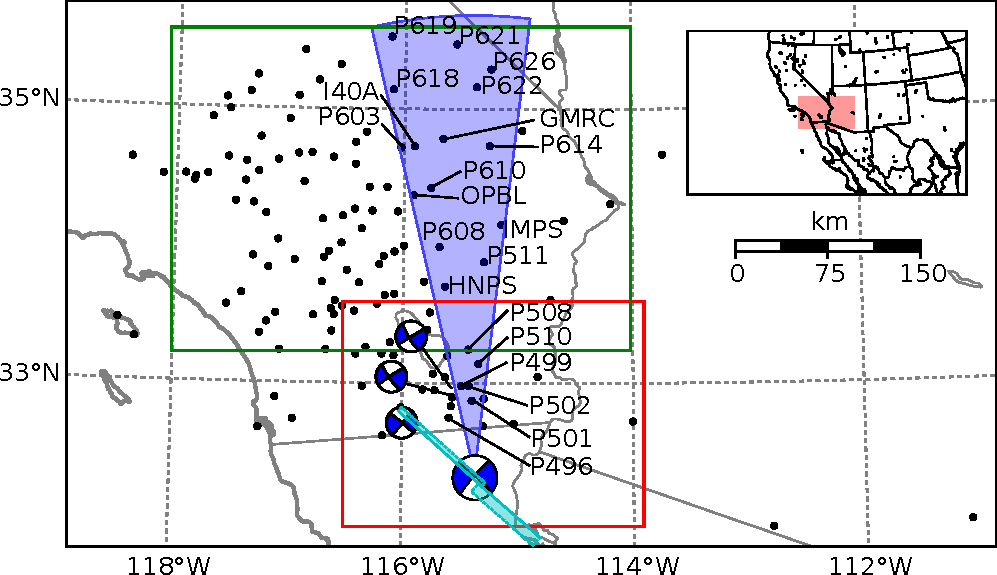
\includegraphics[scale=0.9]{Figures/context_map}
\centering 
\caption{}
\label{ContextMap}
\end{figure}

\begin{figure}
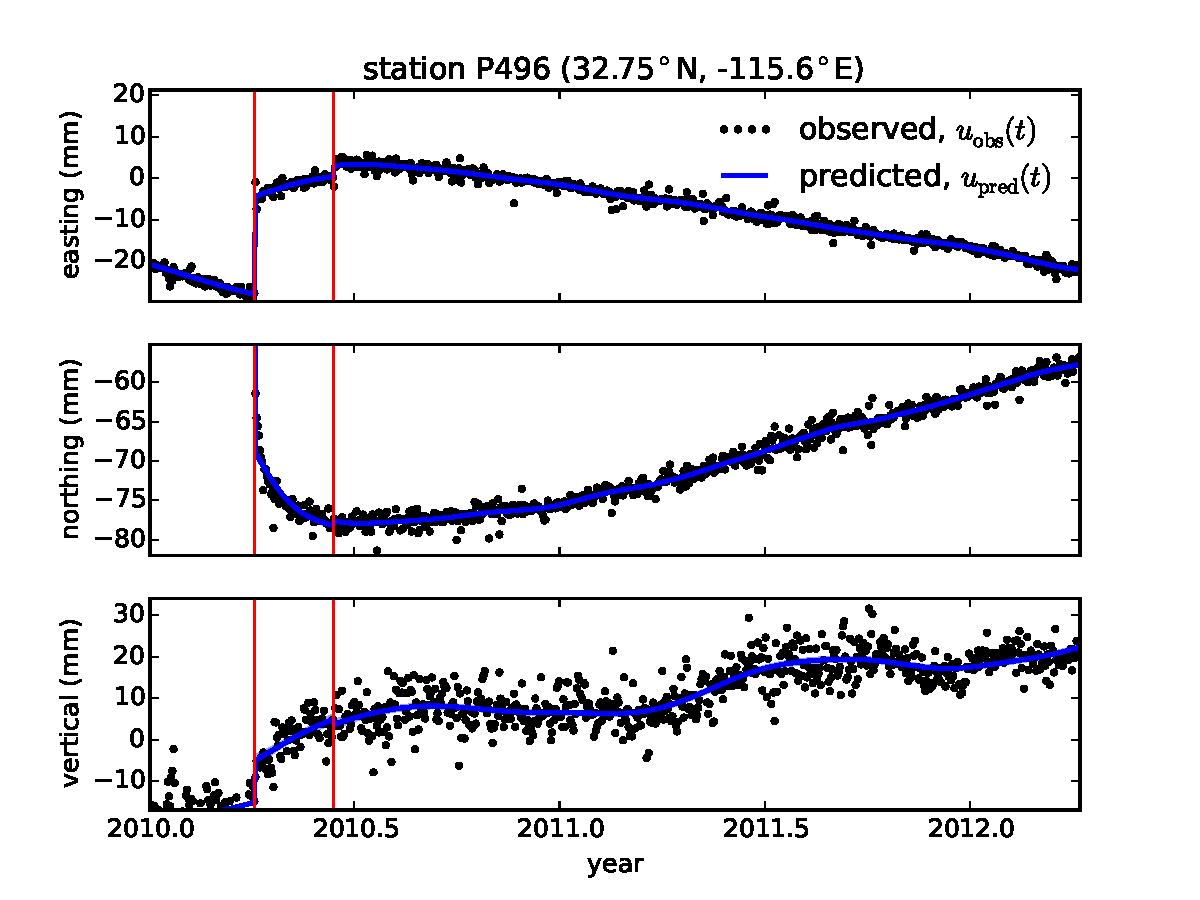
\includegraphics[scale=0.6]{Figures/figure_1}
\centering
\caption{GPS displacement solution from UNAVCO (black) and predicted displacements after applying a Kalman filter where $\sigma^2=0.05 \mathrm{m}^2/\mathrm{yr}^3$. Red line indicates the time of the Ocotillo earthquake where a jump in the time series is estimated}
\label{P496Fit}
\end{figure}

\begin{figure}
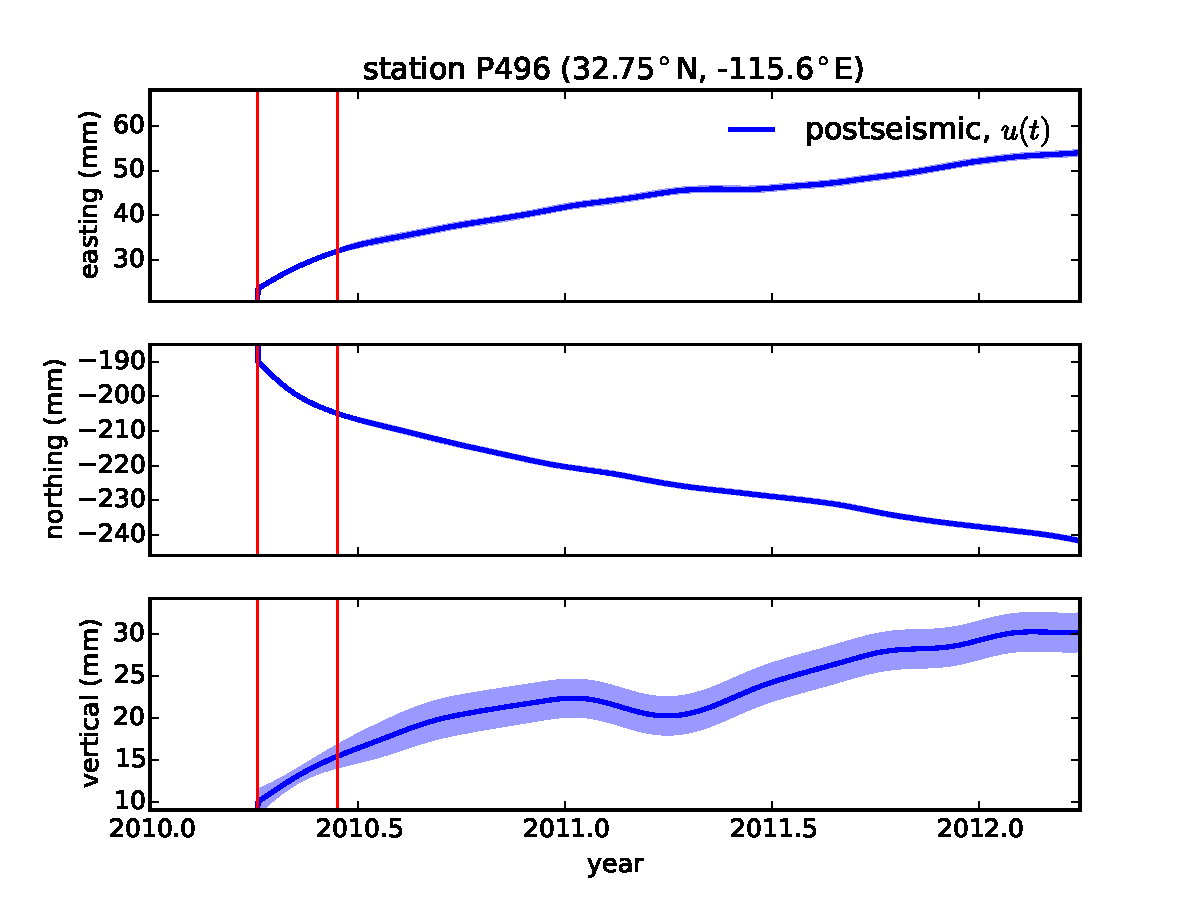
\includegraphics[scale=0.6]{Figures/figure_2}
\centering
\caption{Postseismic displacements estimated after applying a Kalman filter to the GPS displacement solution from UNAVCO.  Displacements shown have had a background secular trend removed as well as an estimated seasonal signal.} 
\label{P496PS}
\end{figure}

\begin{figure}
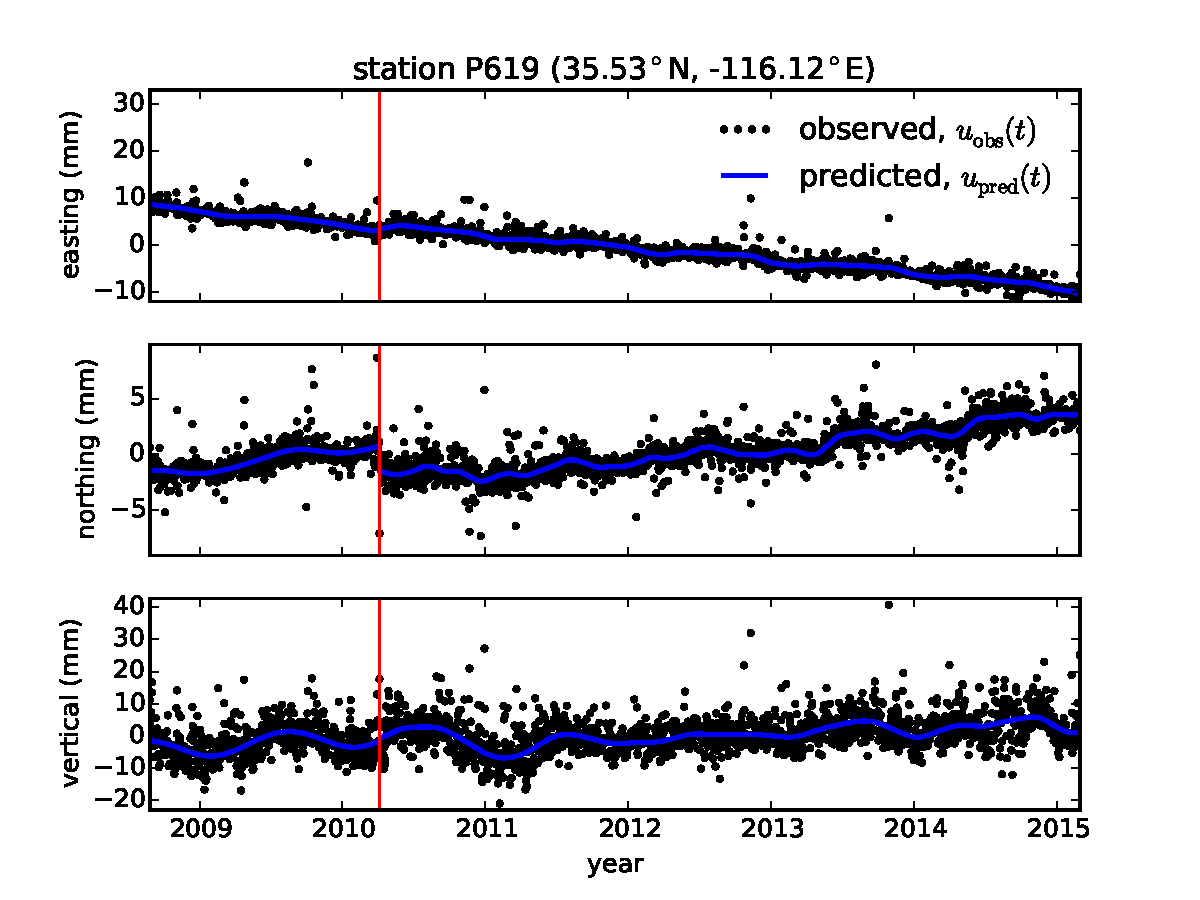
\includegraphics[scale=0.6]{Figures/figure_3}
\centering
\caption{GPS displacement solution from UNAVCO (black) and predicted displacements after applying a Kalman filter where $\sigma^2=0.05 \mathrm{m}^2/\mathrm{yr}^3$. Red line indicates the time of the Ocotillo earthquake where a jump in the time series is estimated}
\label{P619Fit}
\end{figure}

\begin{figure}

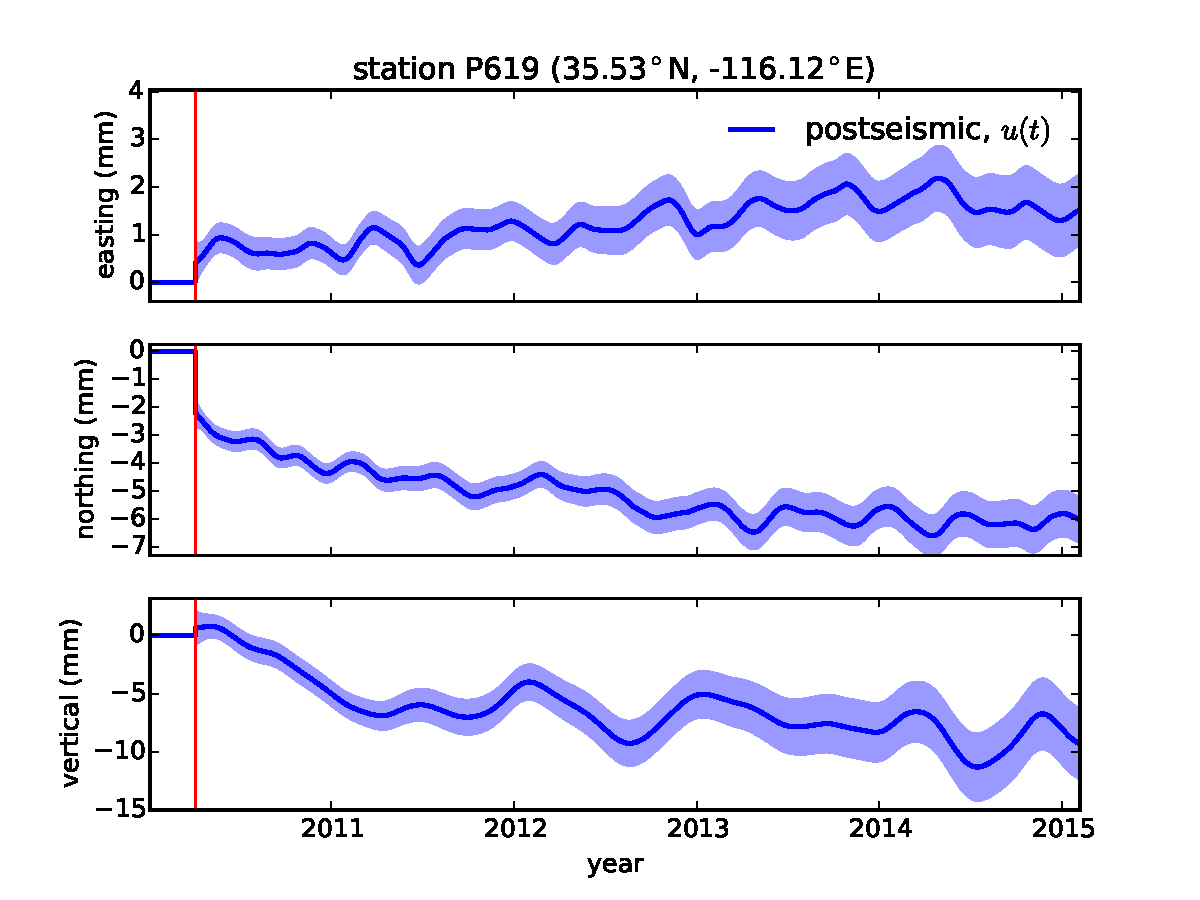
\includegraphics[scale=0.6]{Figures/figure_4}
\centering
\caption{Postseismic displacements estimated after applying a Kalman filter to the GPS displacement solution from UNAVCO.  Displacements shown do not include the estimated secular trend, seasonal signals, and displacements resulting from the Ocotillo earthquake.} 
\label{P619PS}
\end{figure}

\begin{figure}
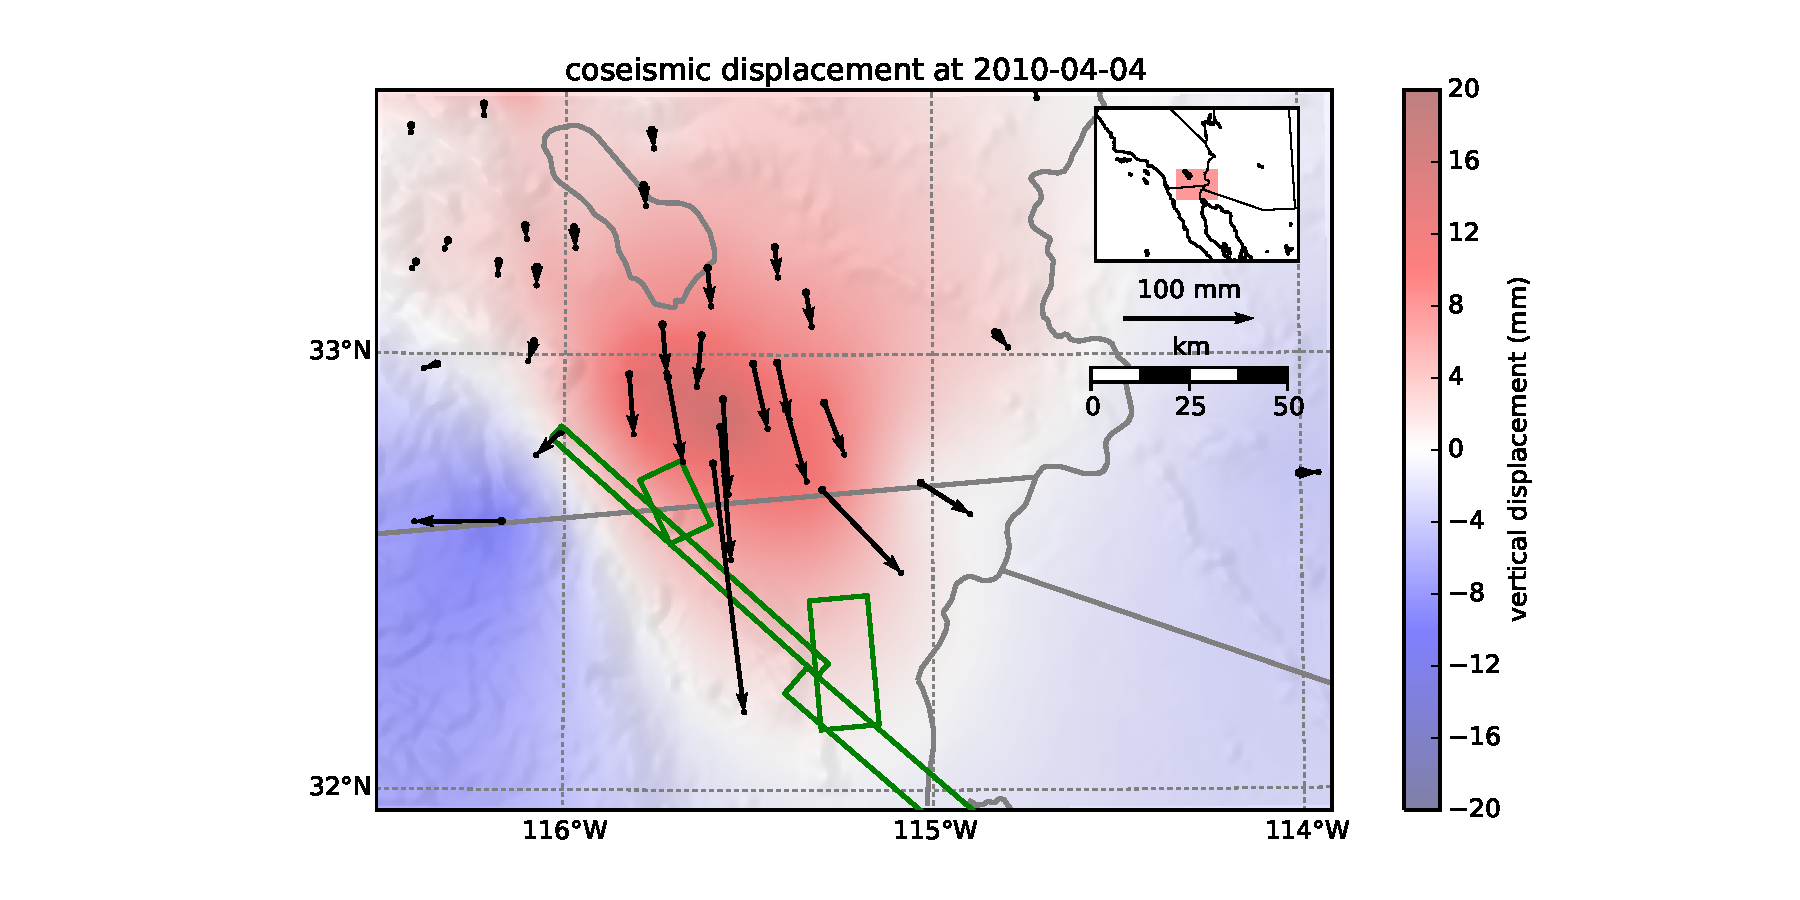
\includegraphics[scale=0.6]{Figures/near_field_data_1}
\centering 
\caption{}
\label{nearfield1}
\end{figure}
\begin{figure}
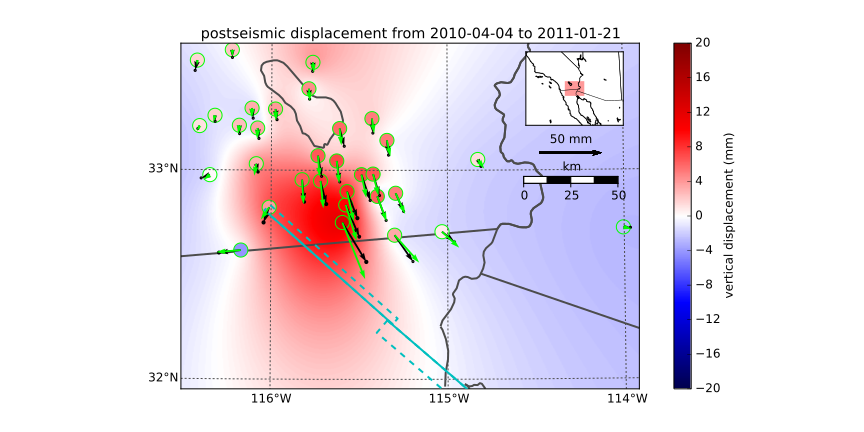
\includegraphics[scale=0.6]{Figures/near_field_data_2}
\centering 
\caption{}
\label{nearfield2}
\end{figure}
\begin{figure}
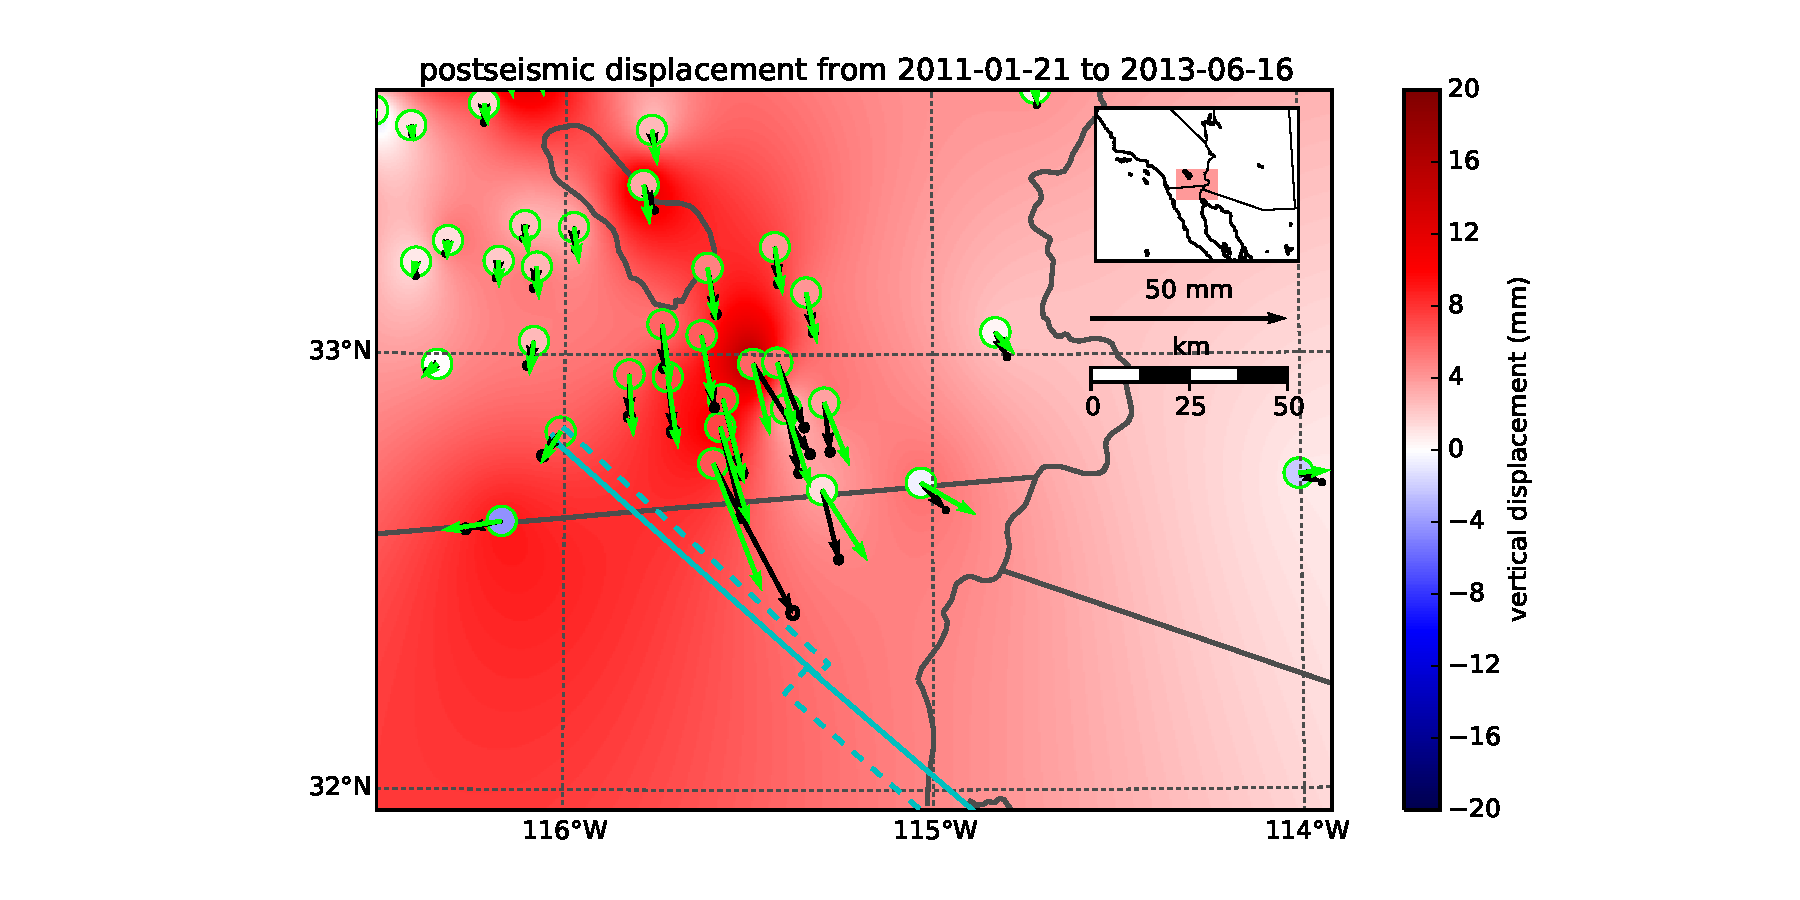
\includegraphics[scale=0.6]{Figures/near_field_data_3}
\centering 
\caption{}
\label{nearfield3}
\end{figure}
\begin{figure}
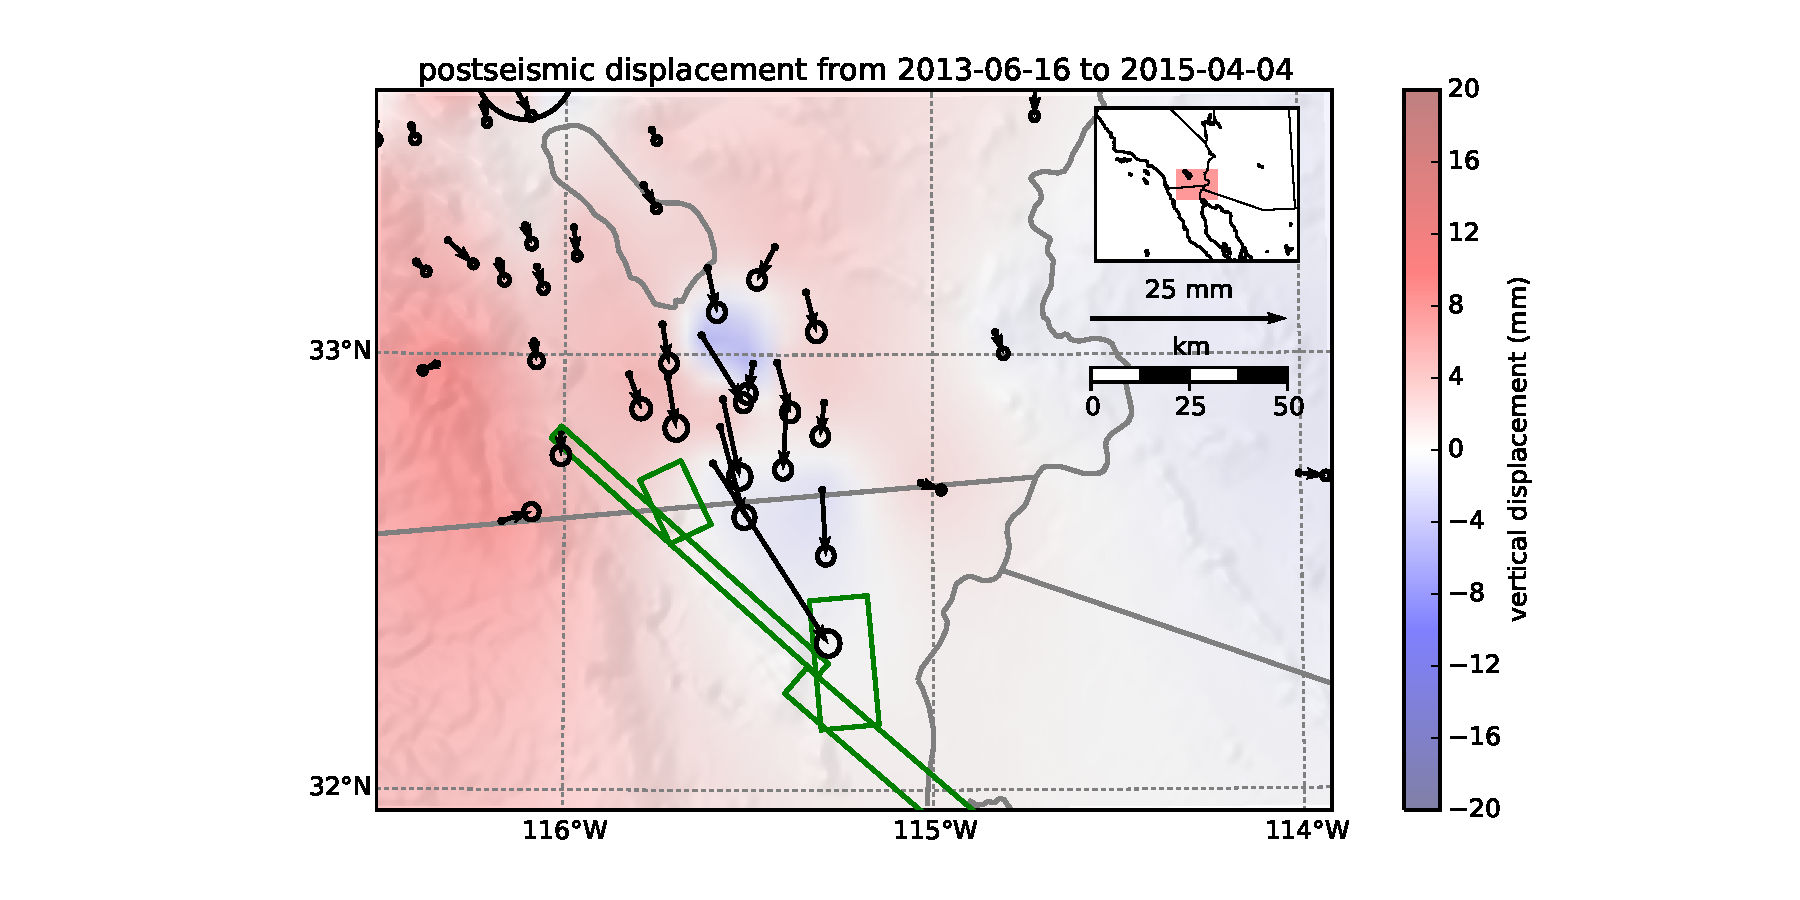
\includegraphics[scale=0.6]{Figures/near_field_data_4}
\centering 
\caption{}
\label{nearfield4}
\end{figure}


\begin{figure}
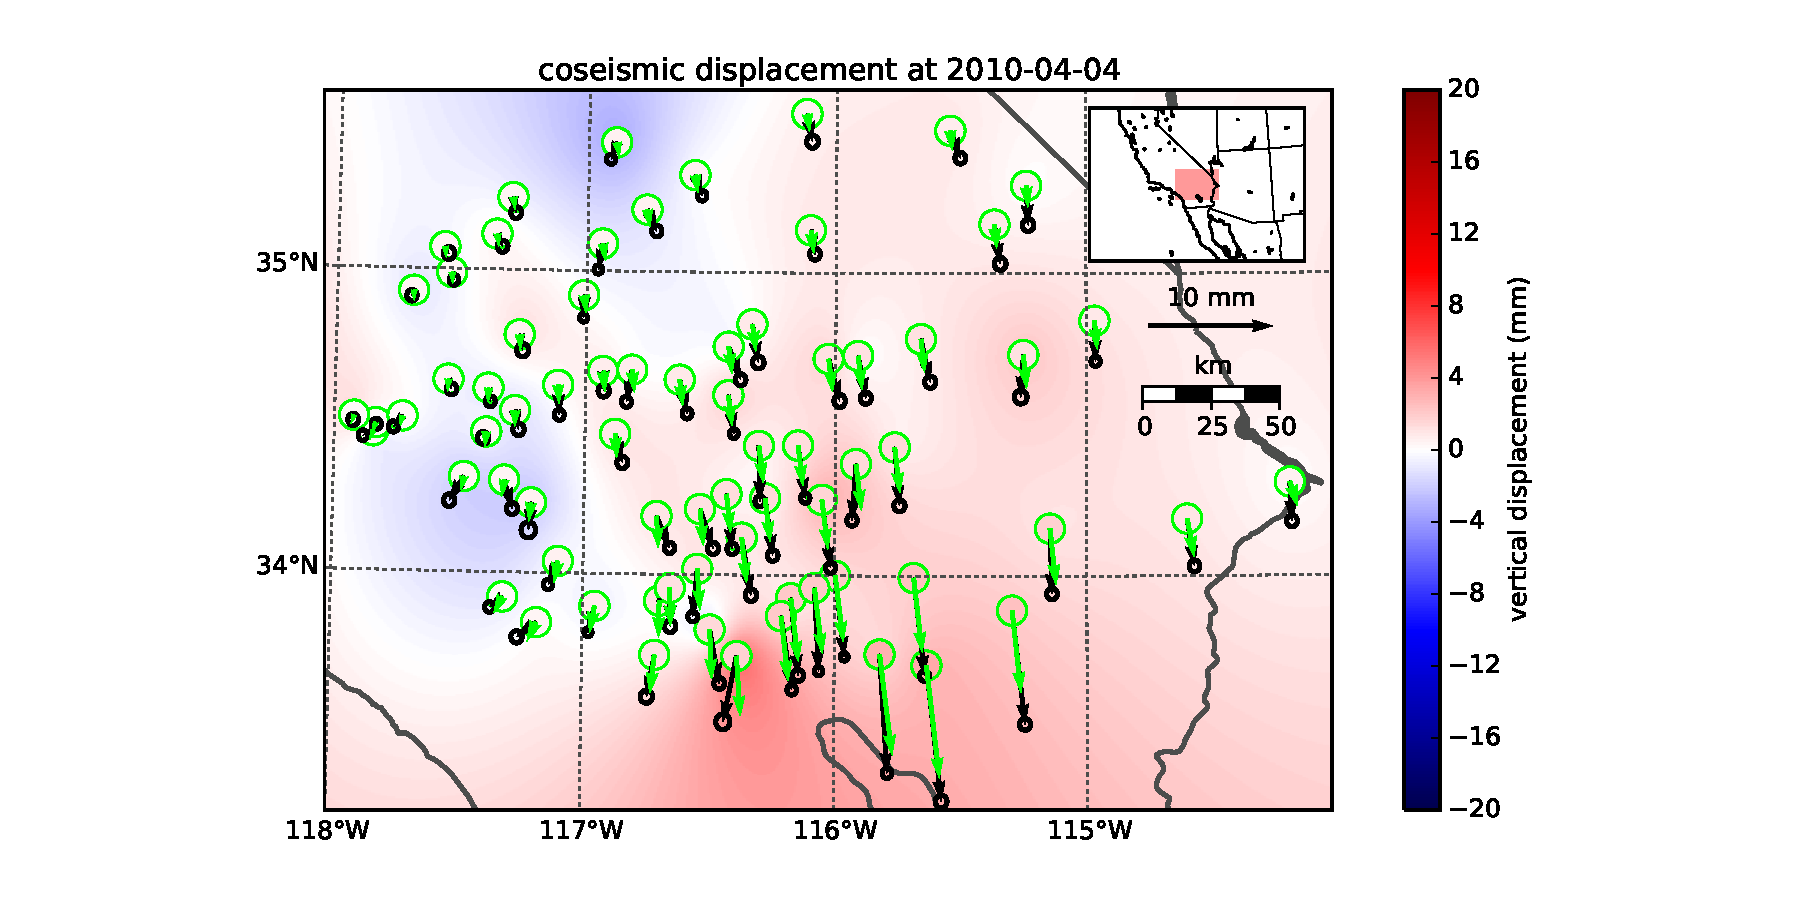
\includegraphics[scale=0.6,resolution=10]{Figures/far_field_data_1}
\centering 
\caption{}
\label{farfield1}
\end{figure}
\begin{figure}
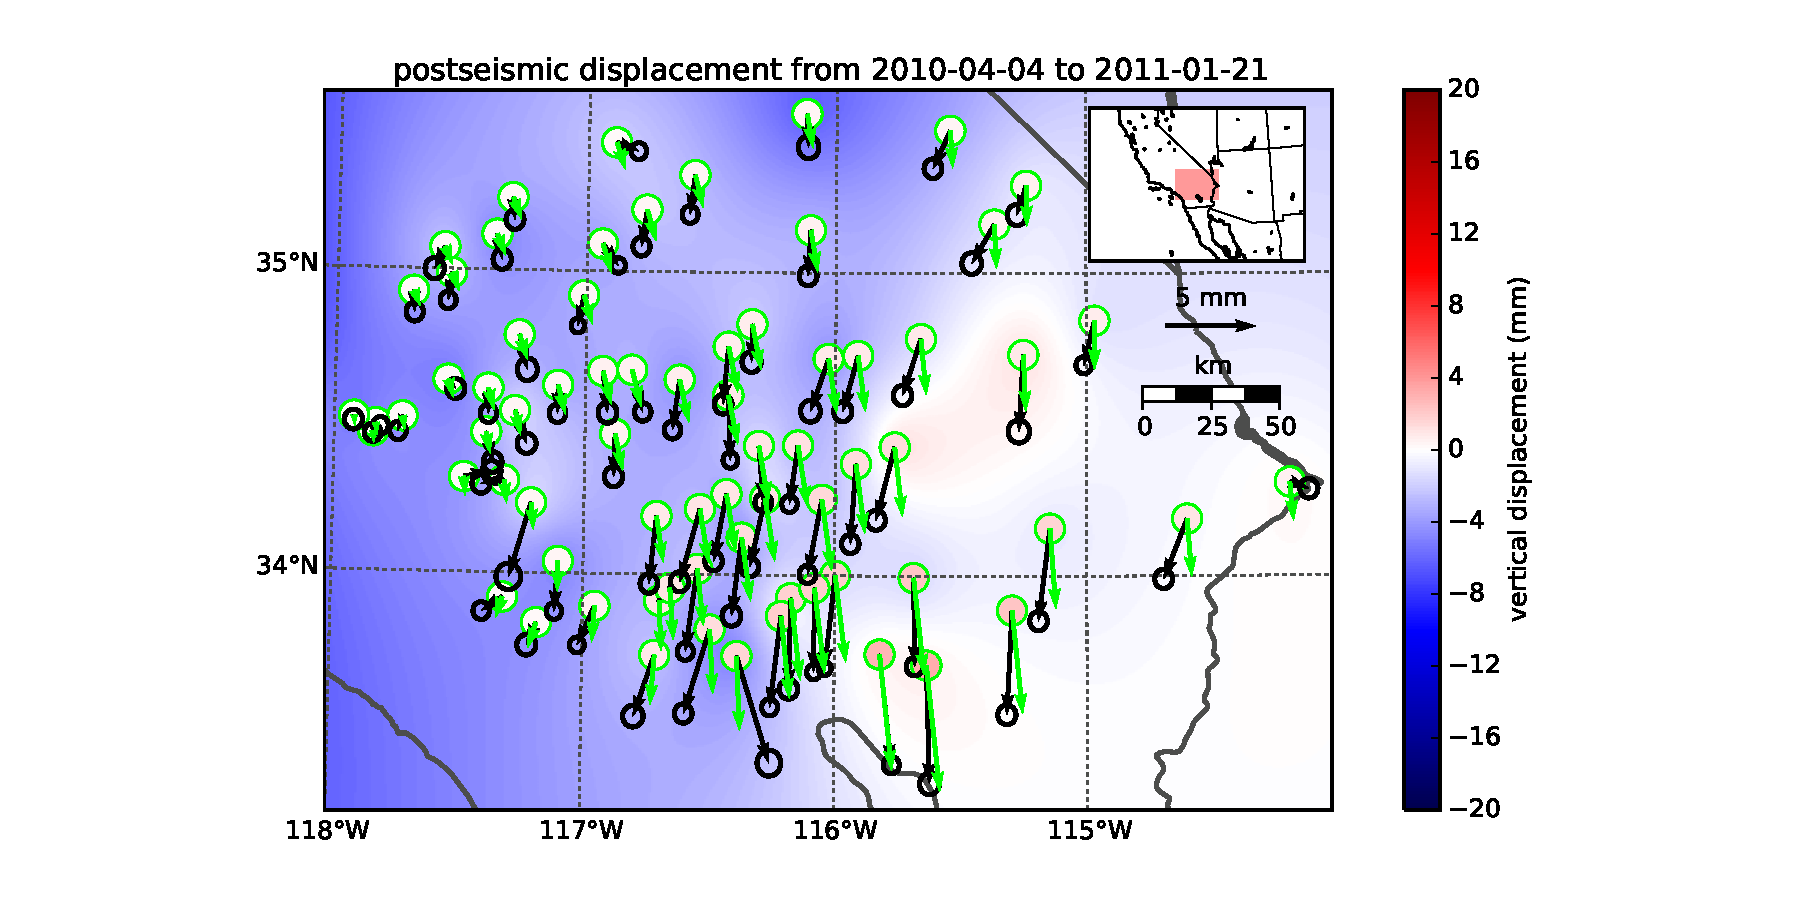
\includegraphics[scale=0.6,resolution=10]{Figures/far_field_data_2}
\centering 
\caption{}
\label{farfield2}
\end{figure}
\begin{figure}
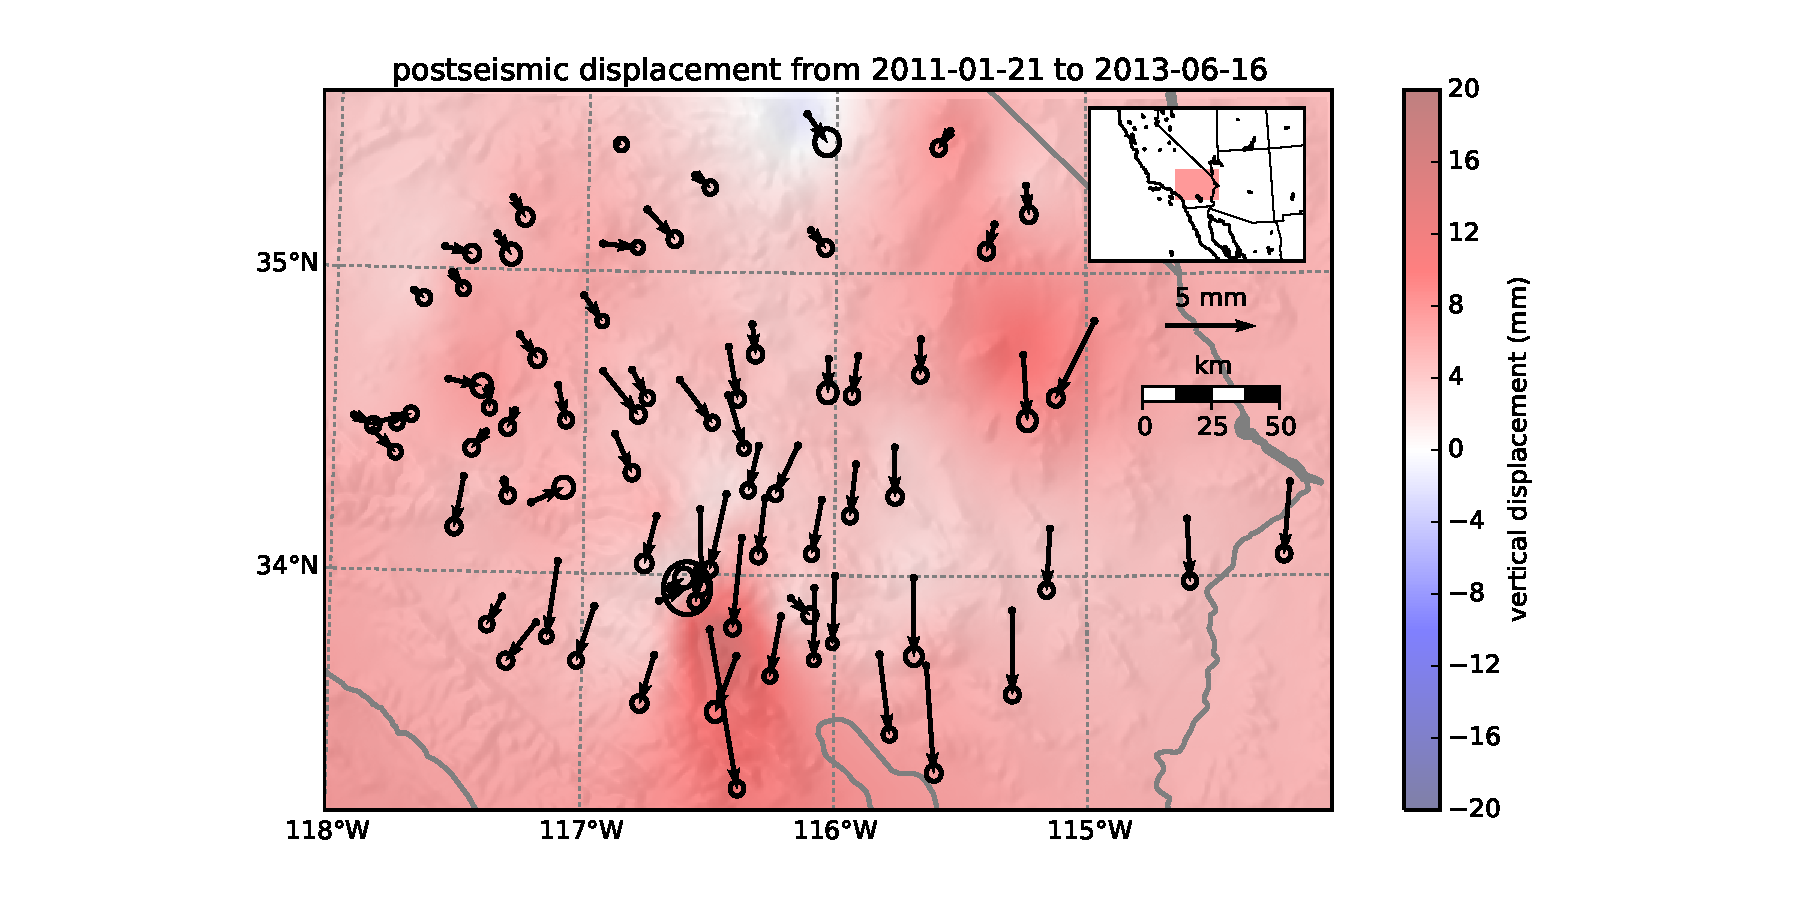
\includegraphics[scale=0.6,resolution=10]{Figures/far_field_data_3}
\centering 
\caption{}
\label{farfield3}
\end{figure}
\begin{figure}
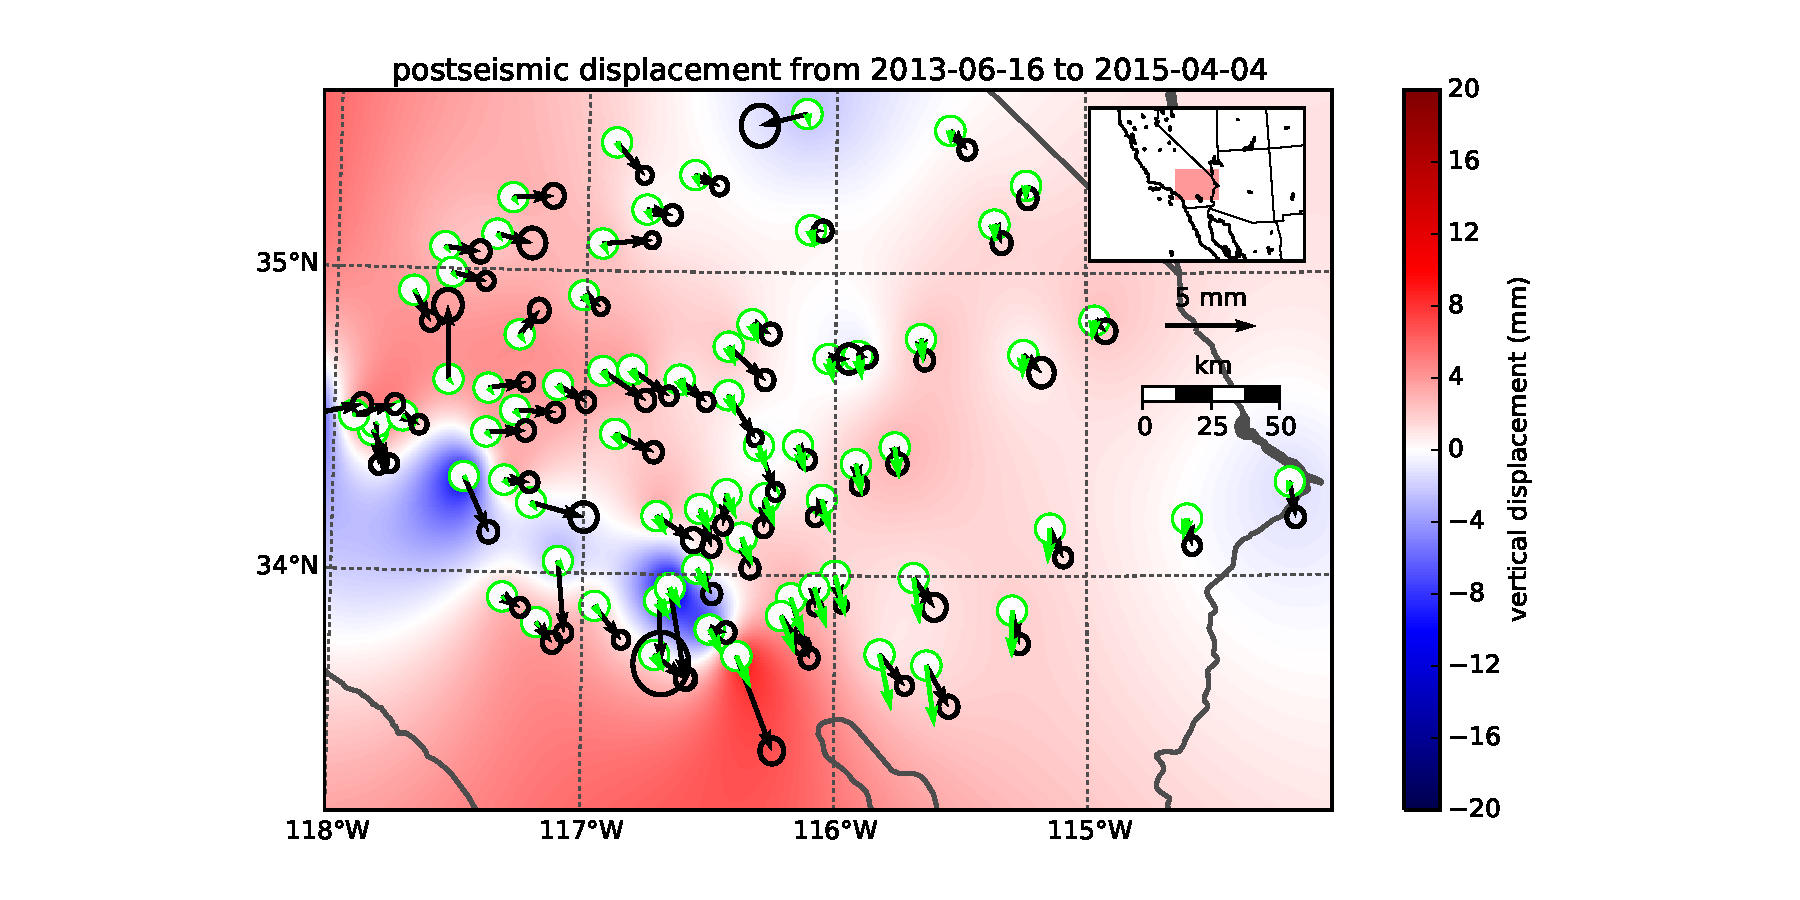
\includegraphics[scale=0.6,resolution=10]{Figures/far_field_data_4}
\centering 
\caption{}
\label{farfield4}
\end{figure}

\begin{figure}
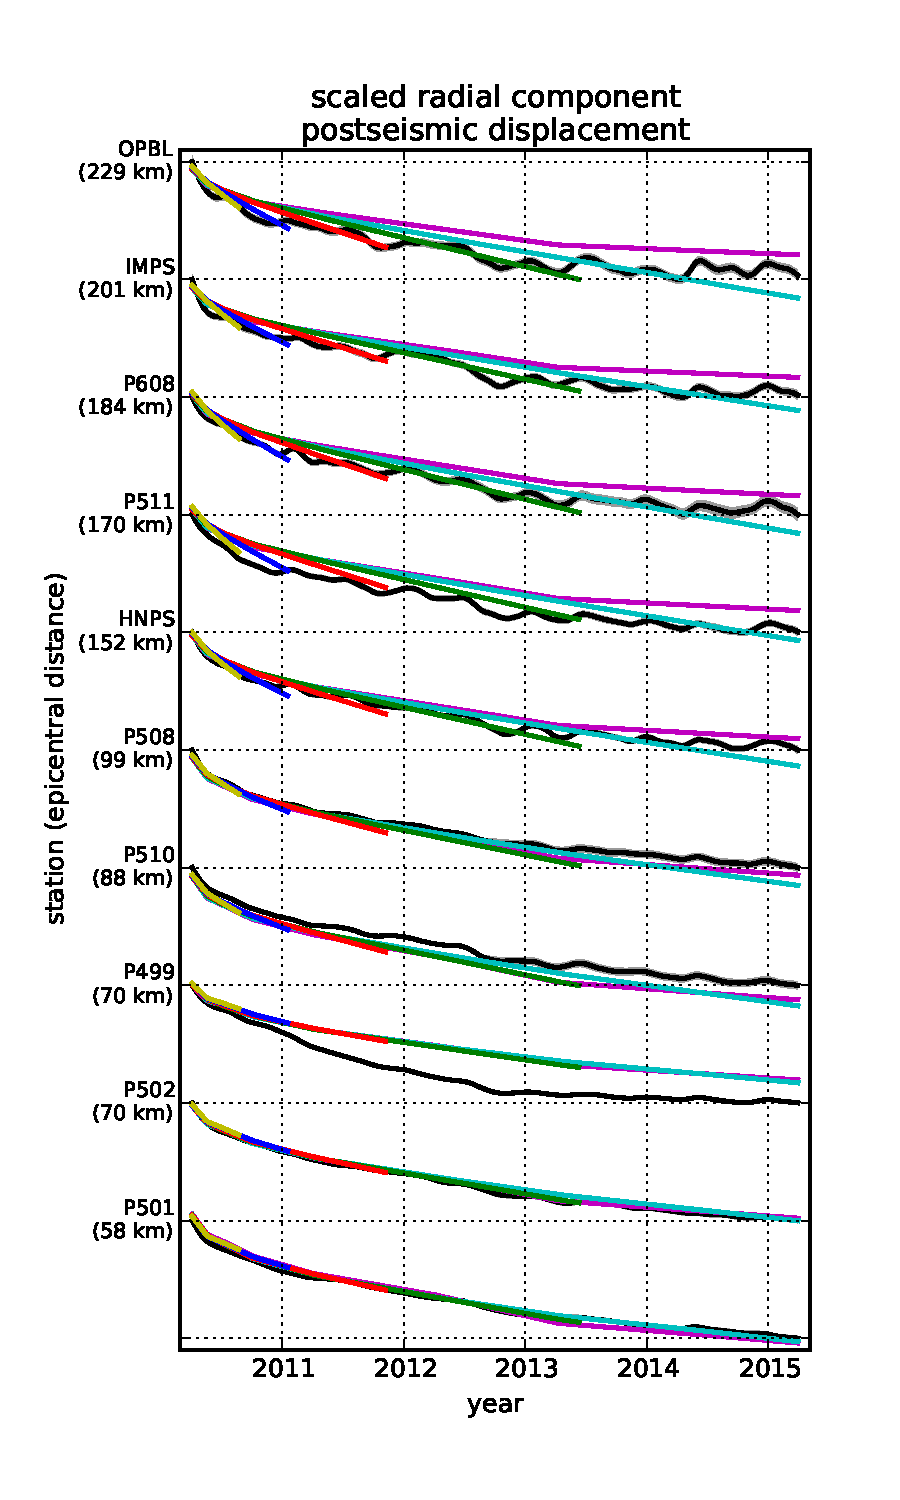
\includegraphics[scale=0.9]{Figures/near_field_record_section}
\centering 
\caption{near field record section}
\label{NearFieldRS}
\end{figure}
\begin{figure}
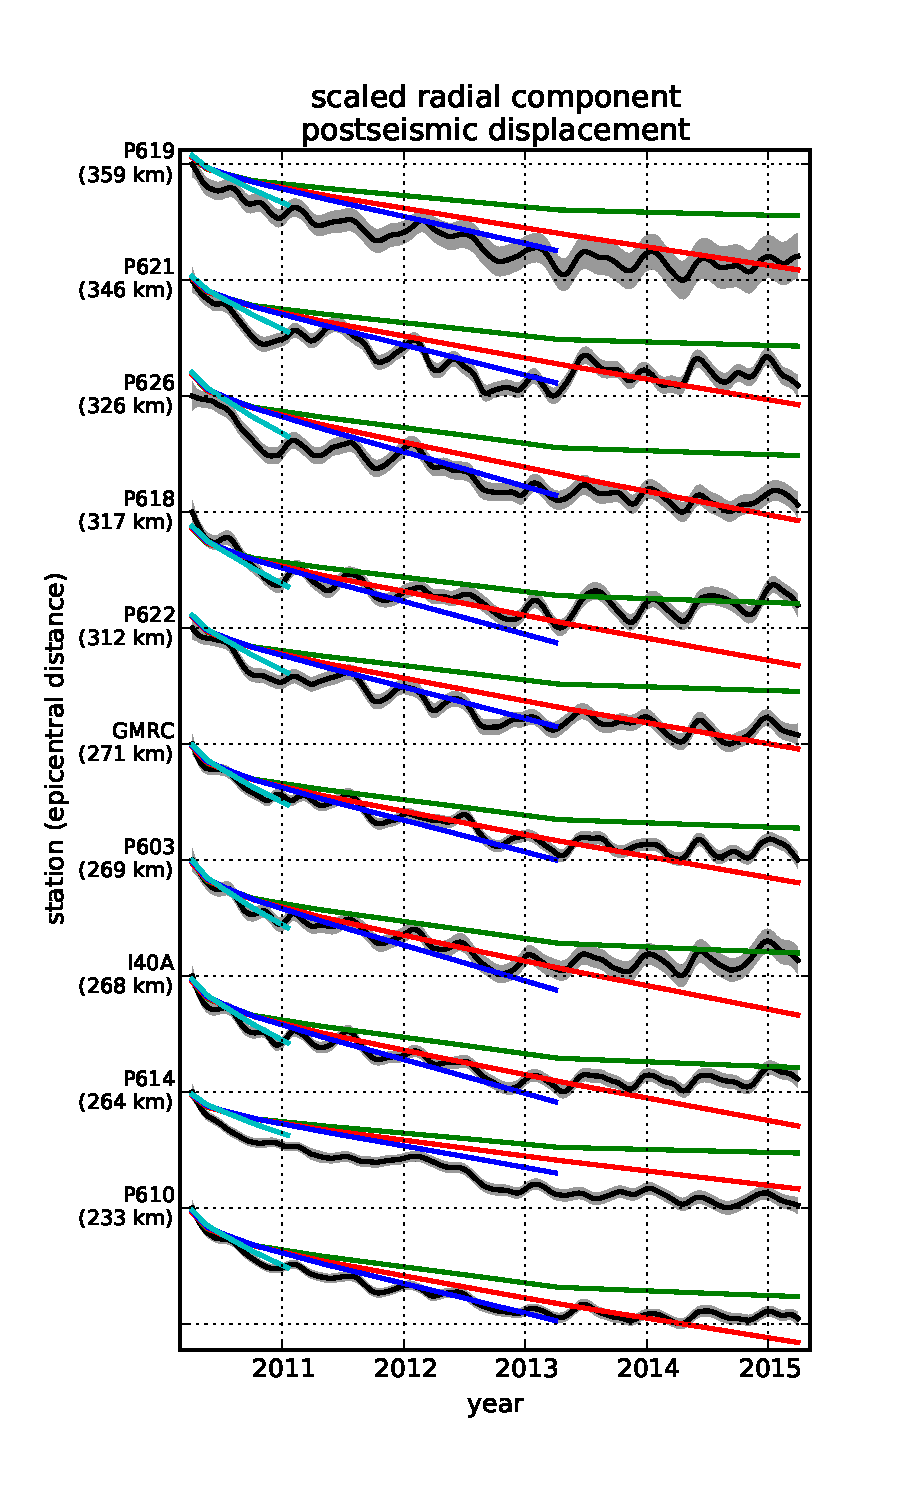
\includegraphics[scale=0.9]{Figures/far_field_record_section}
\centering 
\caption{far field record section}
\label{FarFieldRS}
\end{figure}        
\begin{figure}

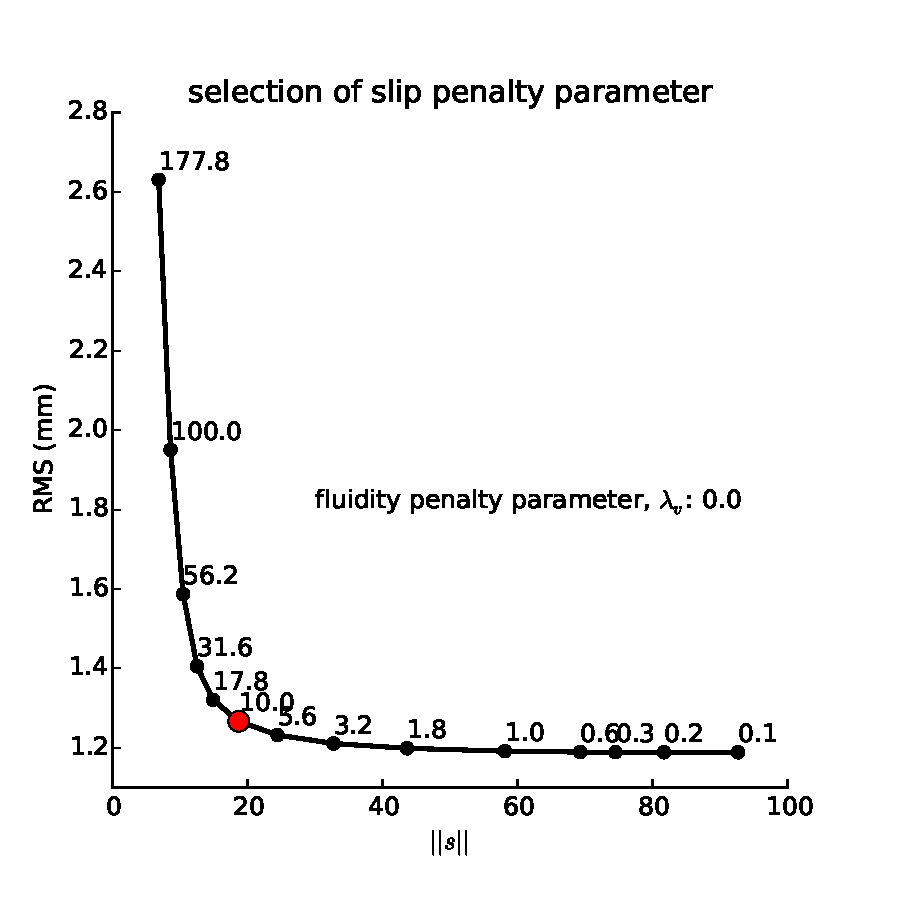
\includegraphics[scale=1.0]{Figures/slip_lcurve}
\centering 
\caption{near field record section}
\label{SlipLCurve}
\end{figure}

\begin{figure}
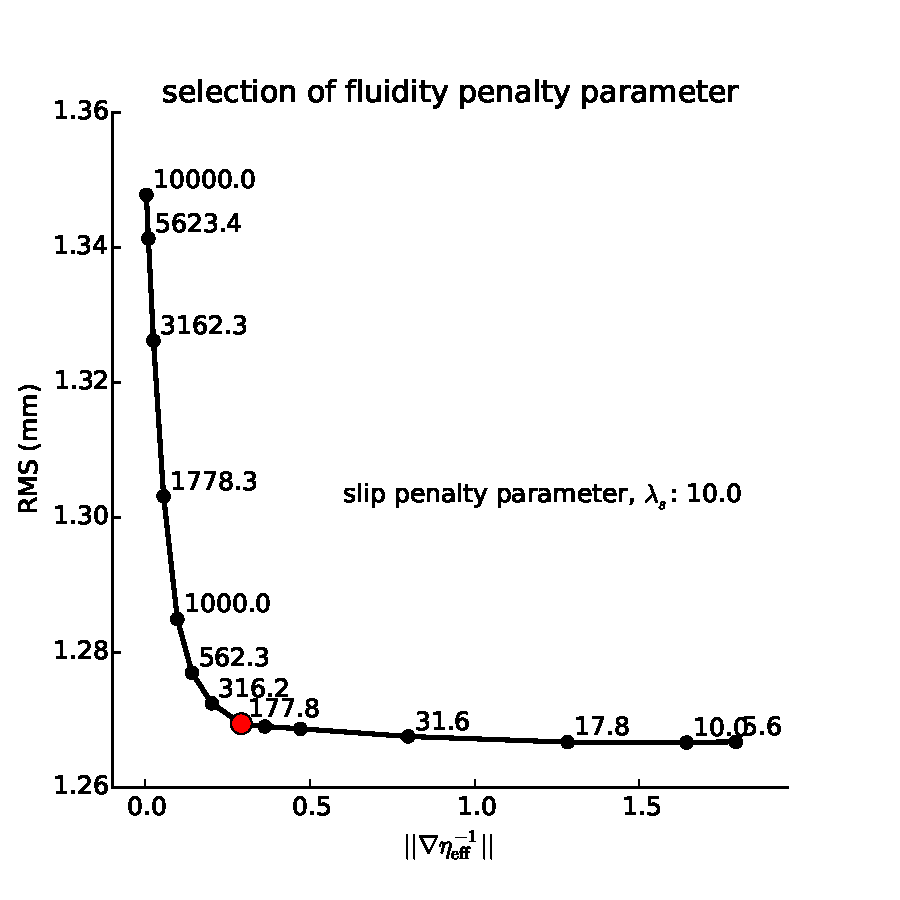
\includegraphics[scale=1.0]{Figures/fluidity_lcurve}
\centering 
\caption{far field record section}
\label{FluidityLCurve}
\end{figure} 

\begin{figure}
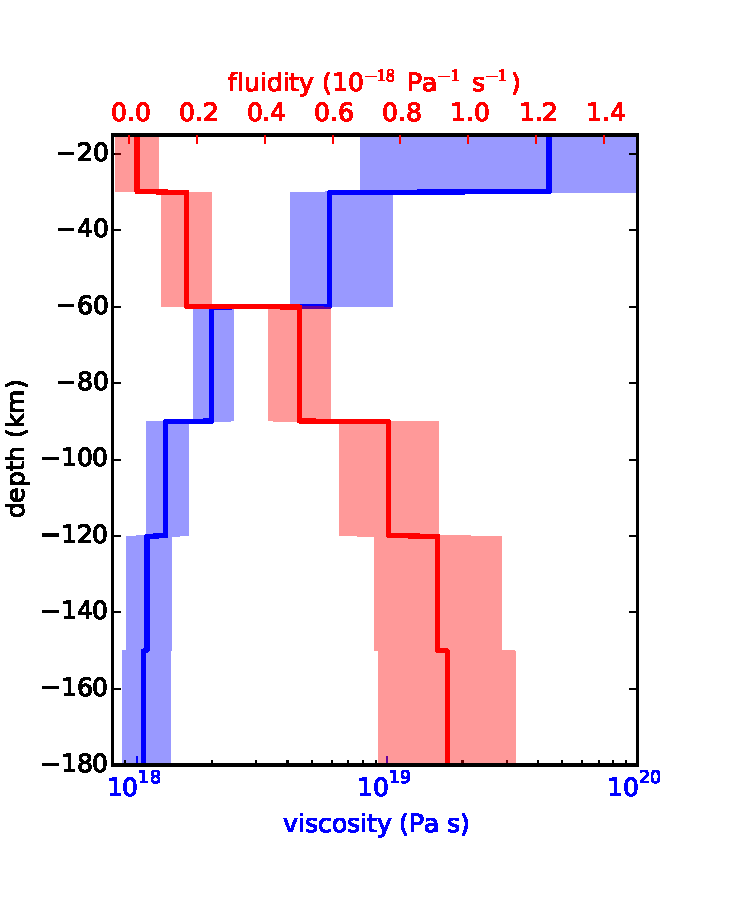
\includegraphics[scale=1.0]{Figures/effective_viscosity}
\centering 
\caption{effective viscosity}
\label{EffectiveViscosity}
\end{figure} 

\begin{figure}
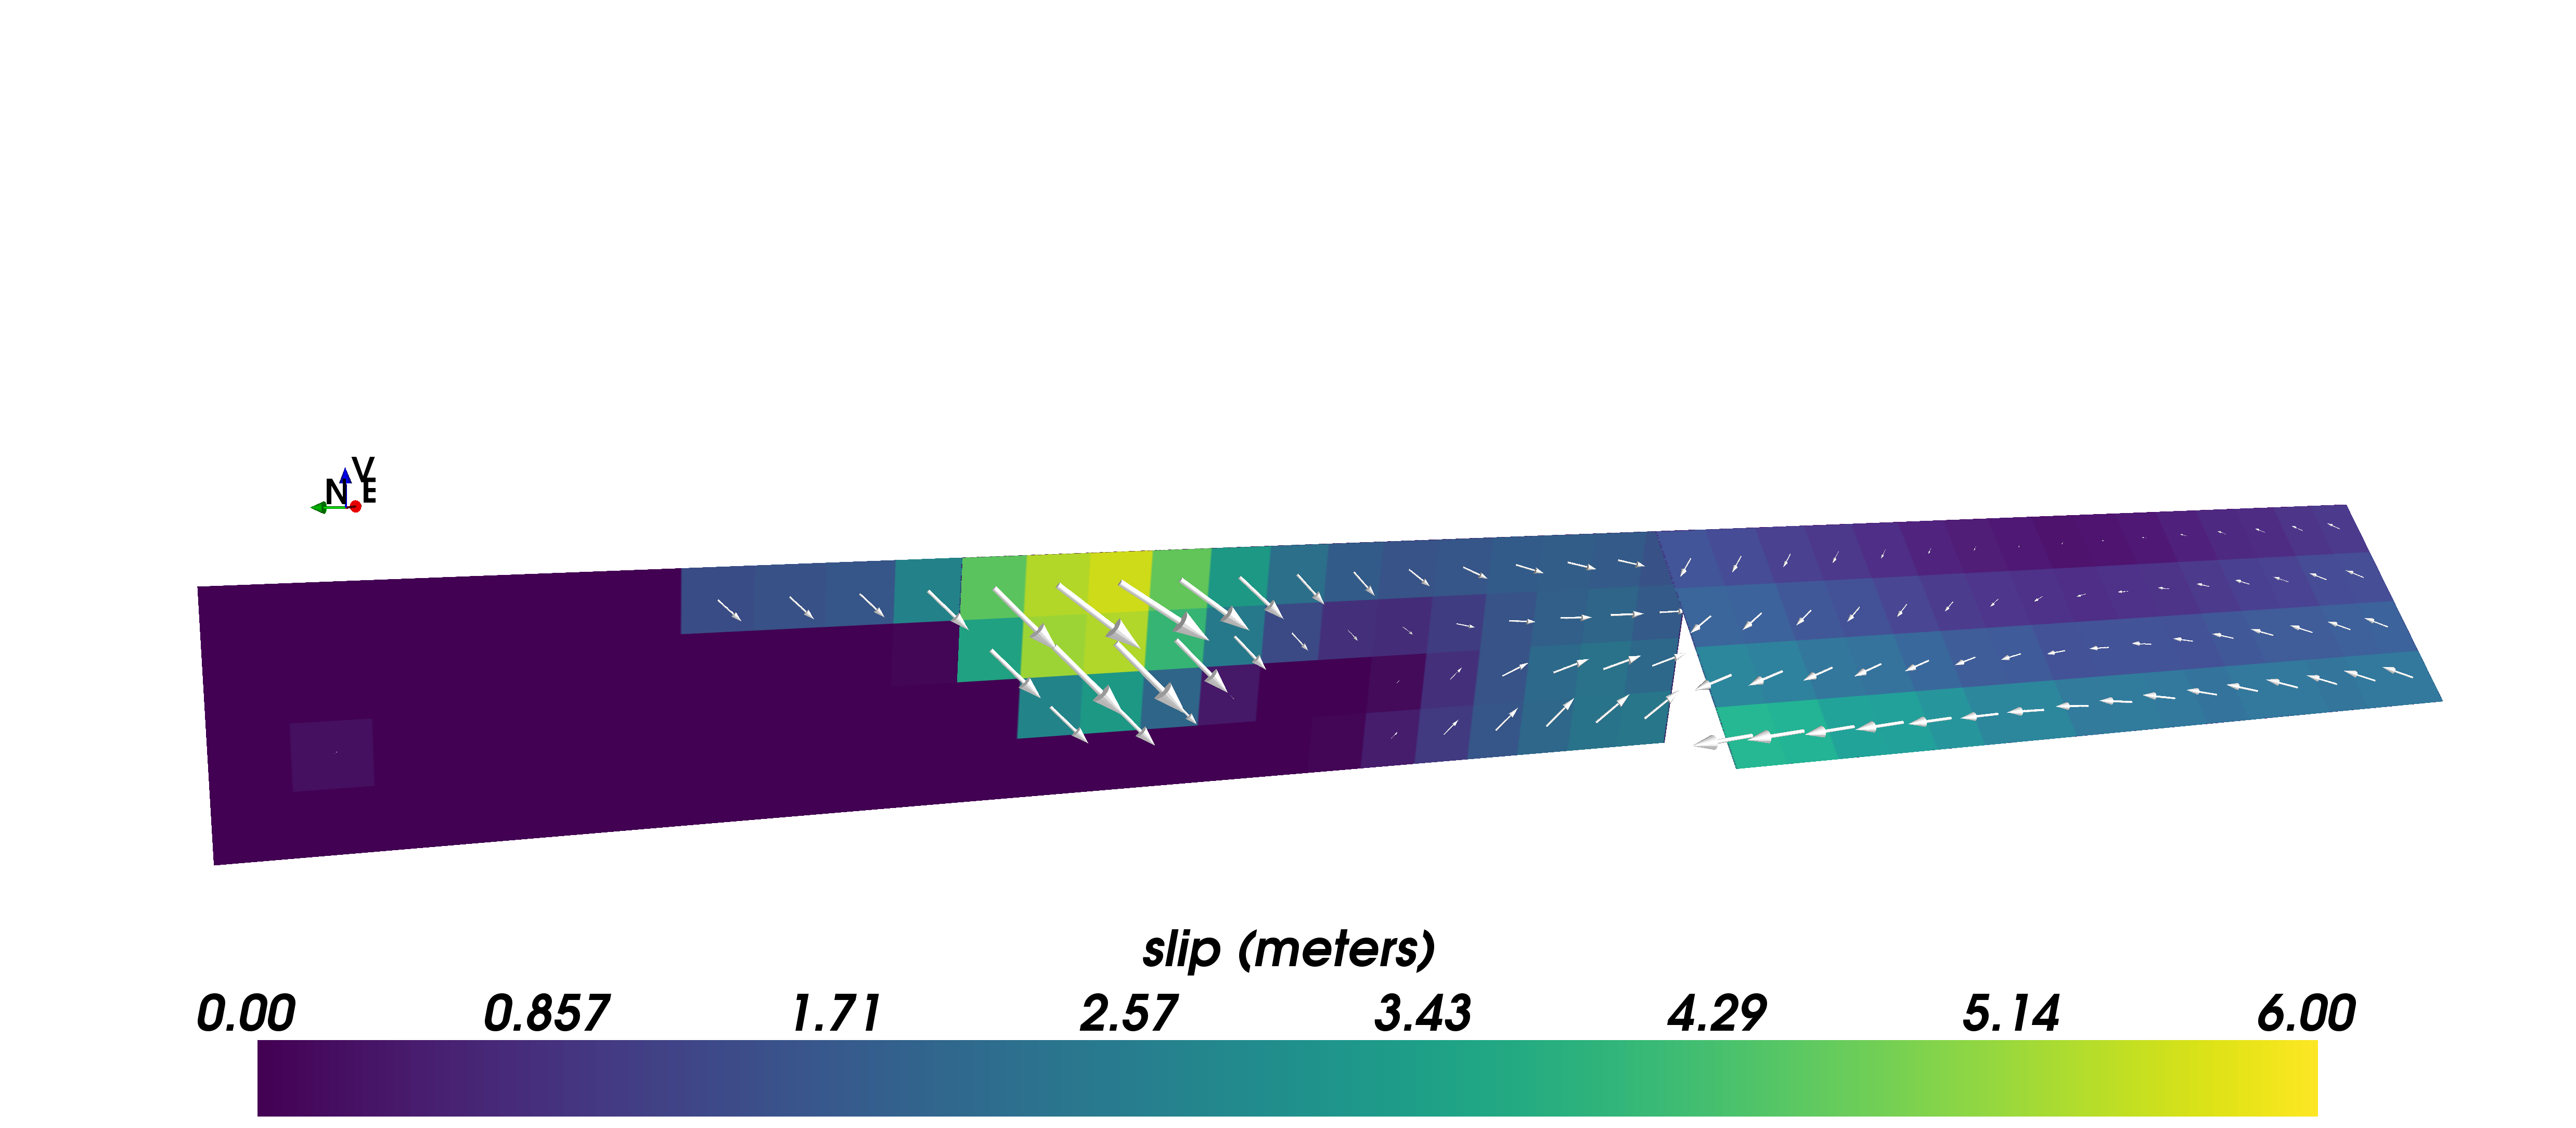
\includegraphics[scale=0.1]{Figures/initial_coseismic}
\caption{coseismic slip from initial inversion}
\label{InitialCoseismic}
\end{figure} 

\begin{figure}
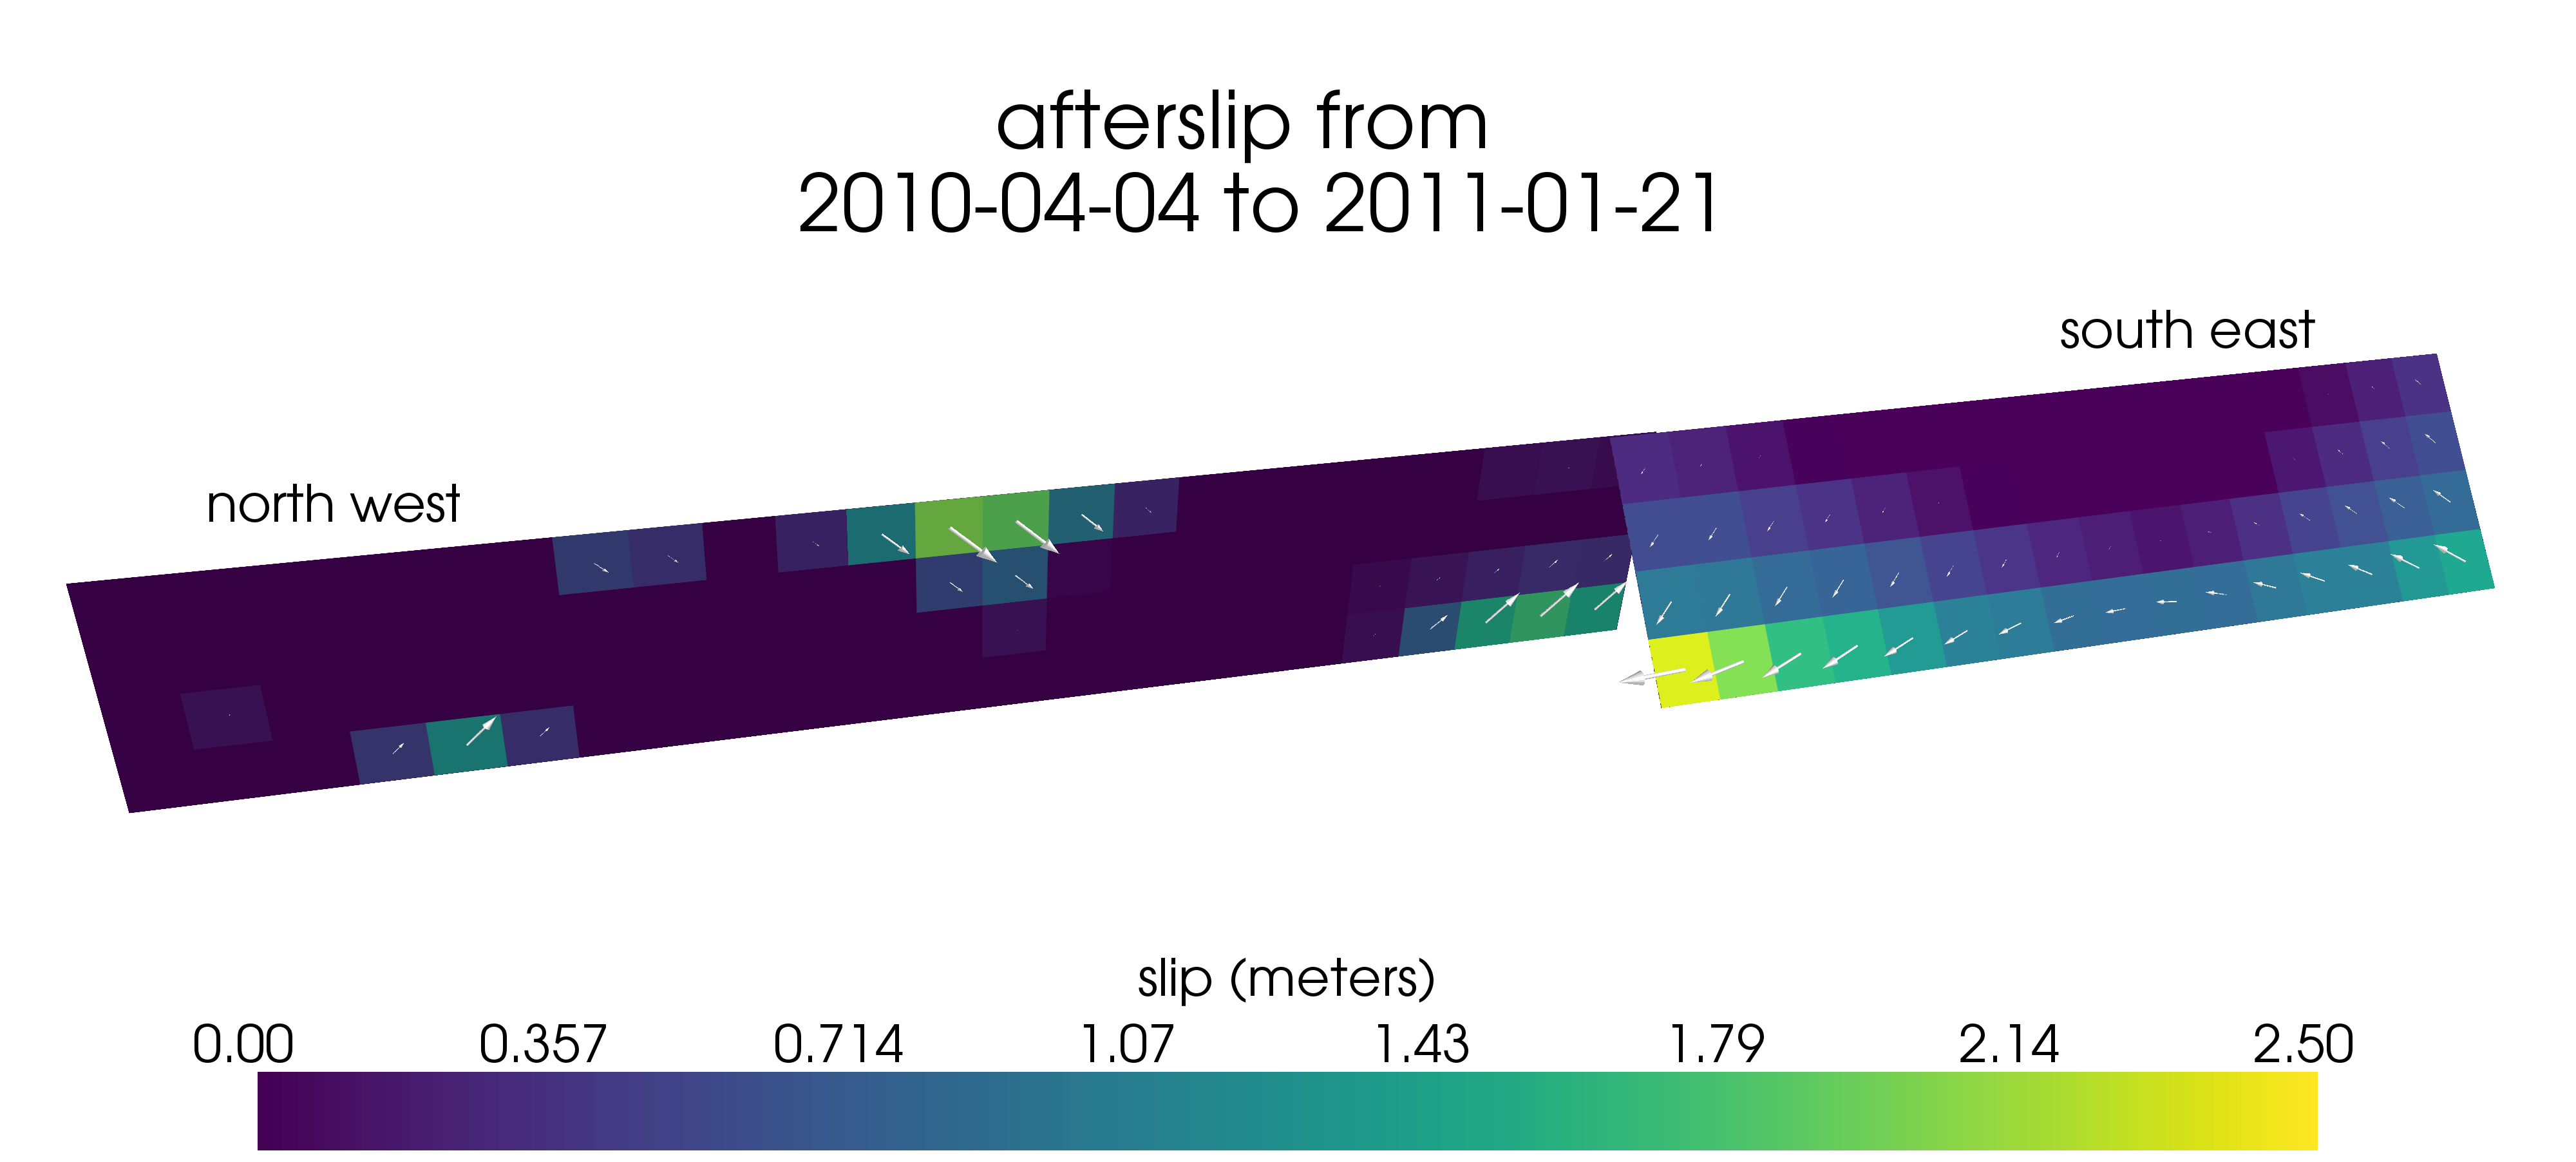
\includegraphics[scale=0.1]{Figures/initial_afterslip}
\centering 
\caption{afterslip from initial inversion}
\label{InitialAfterslip}
\end{figure} 

\begin{figure}
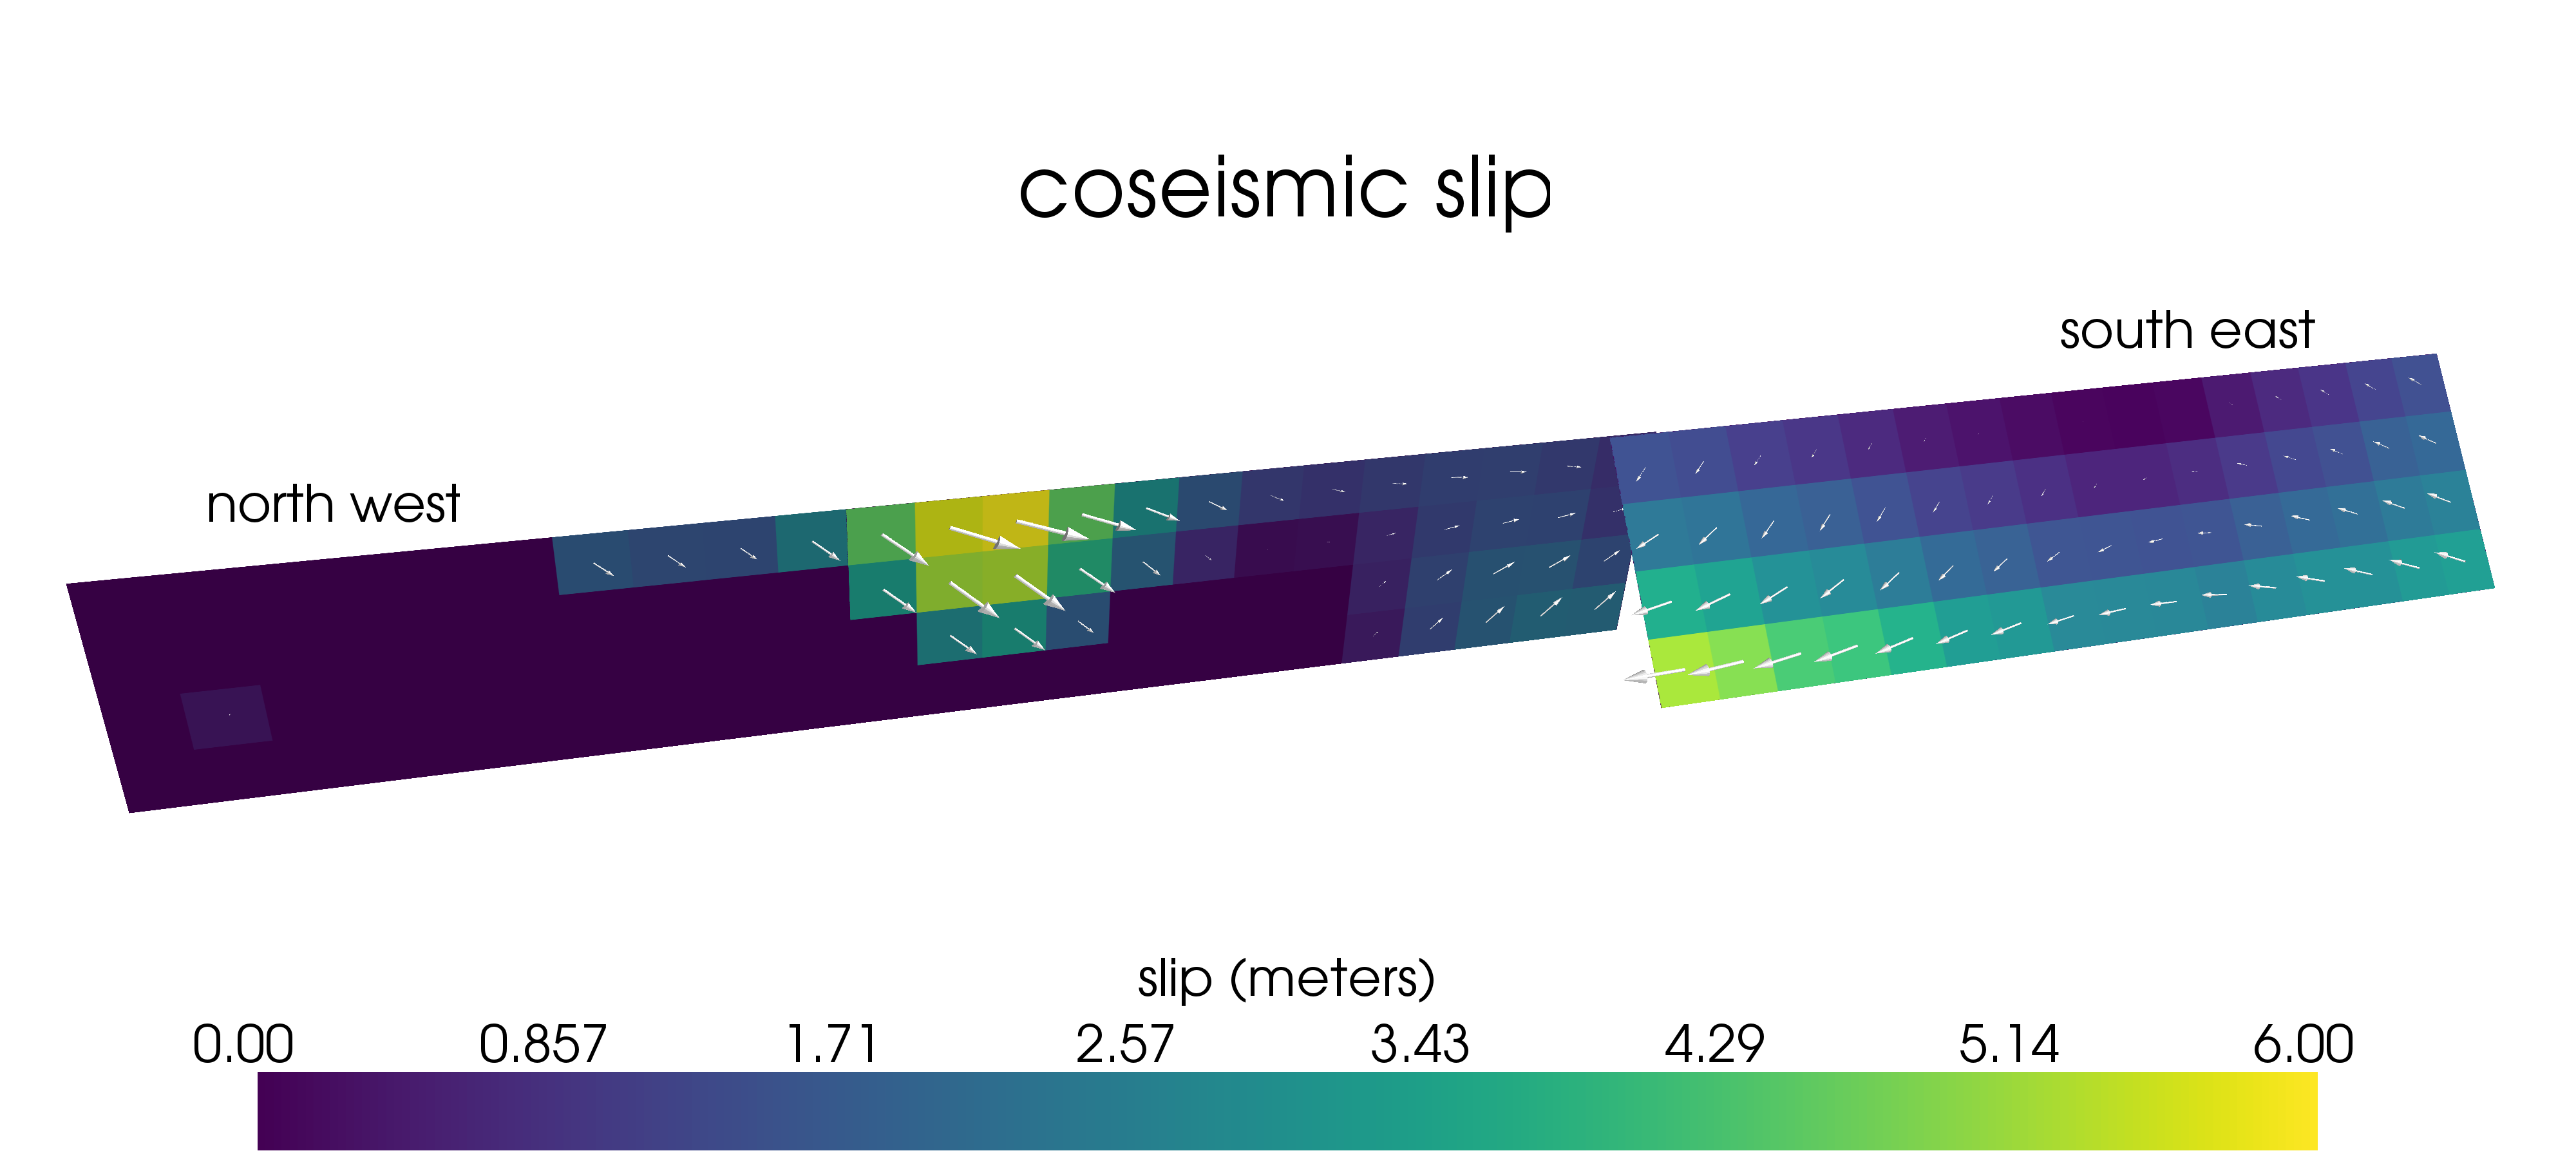
\includegraphics[scale=0.1]{Figures/initial_elastic_coseismic}
\centering 
\caption{coseismic slip from elastic inversion}
\label{InitialElasticCoseismic}
\end{figure} 

\begin{figure}
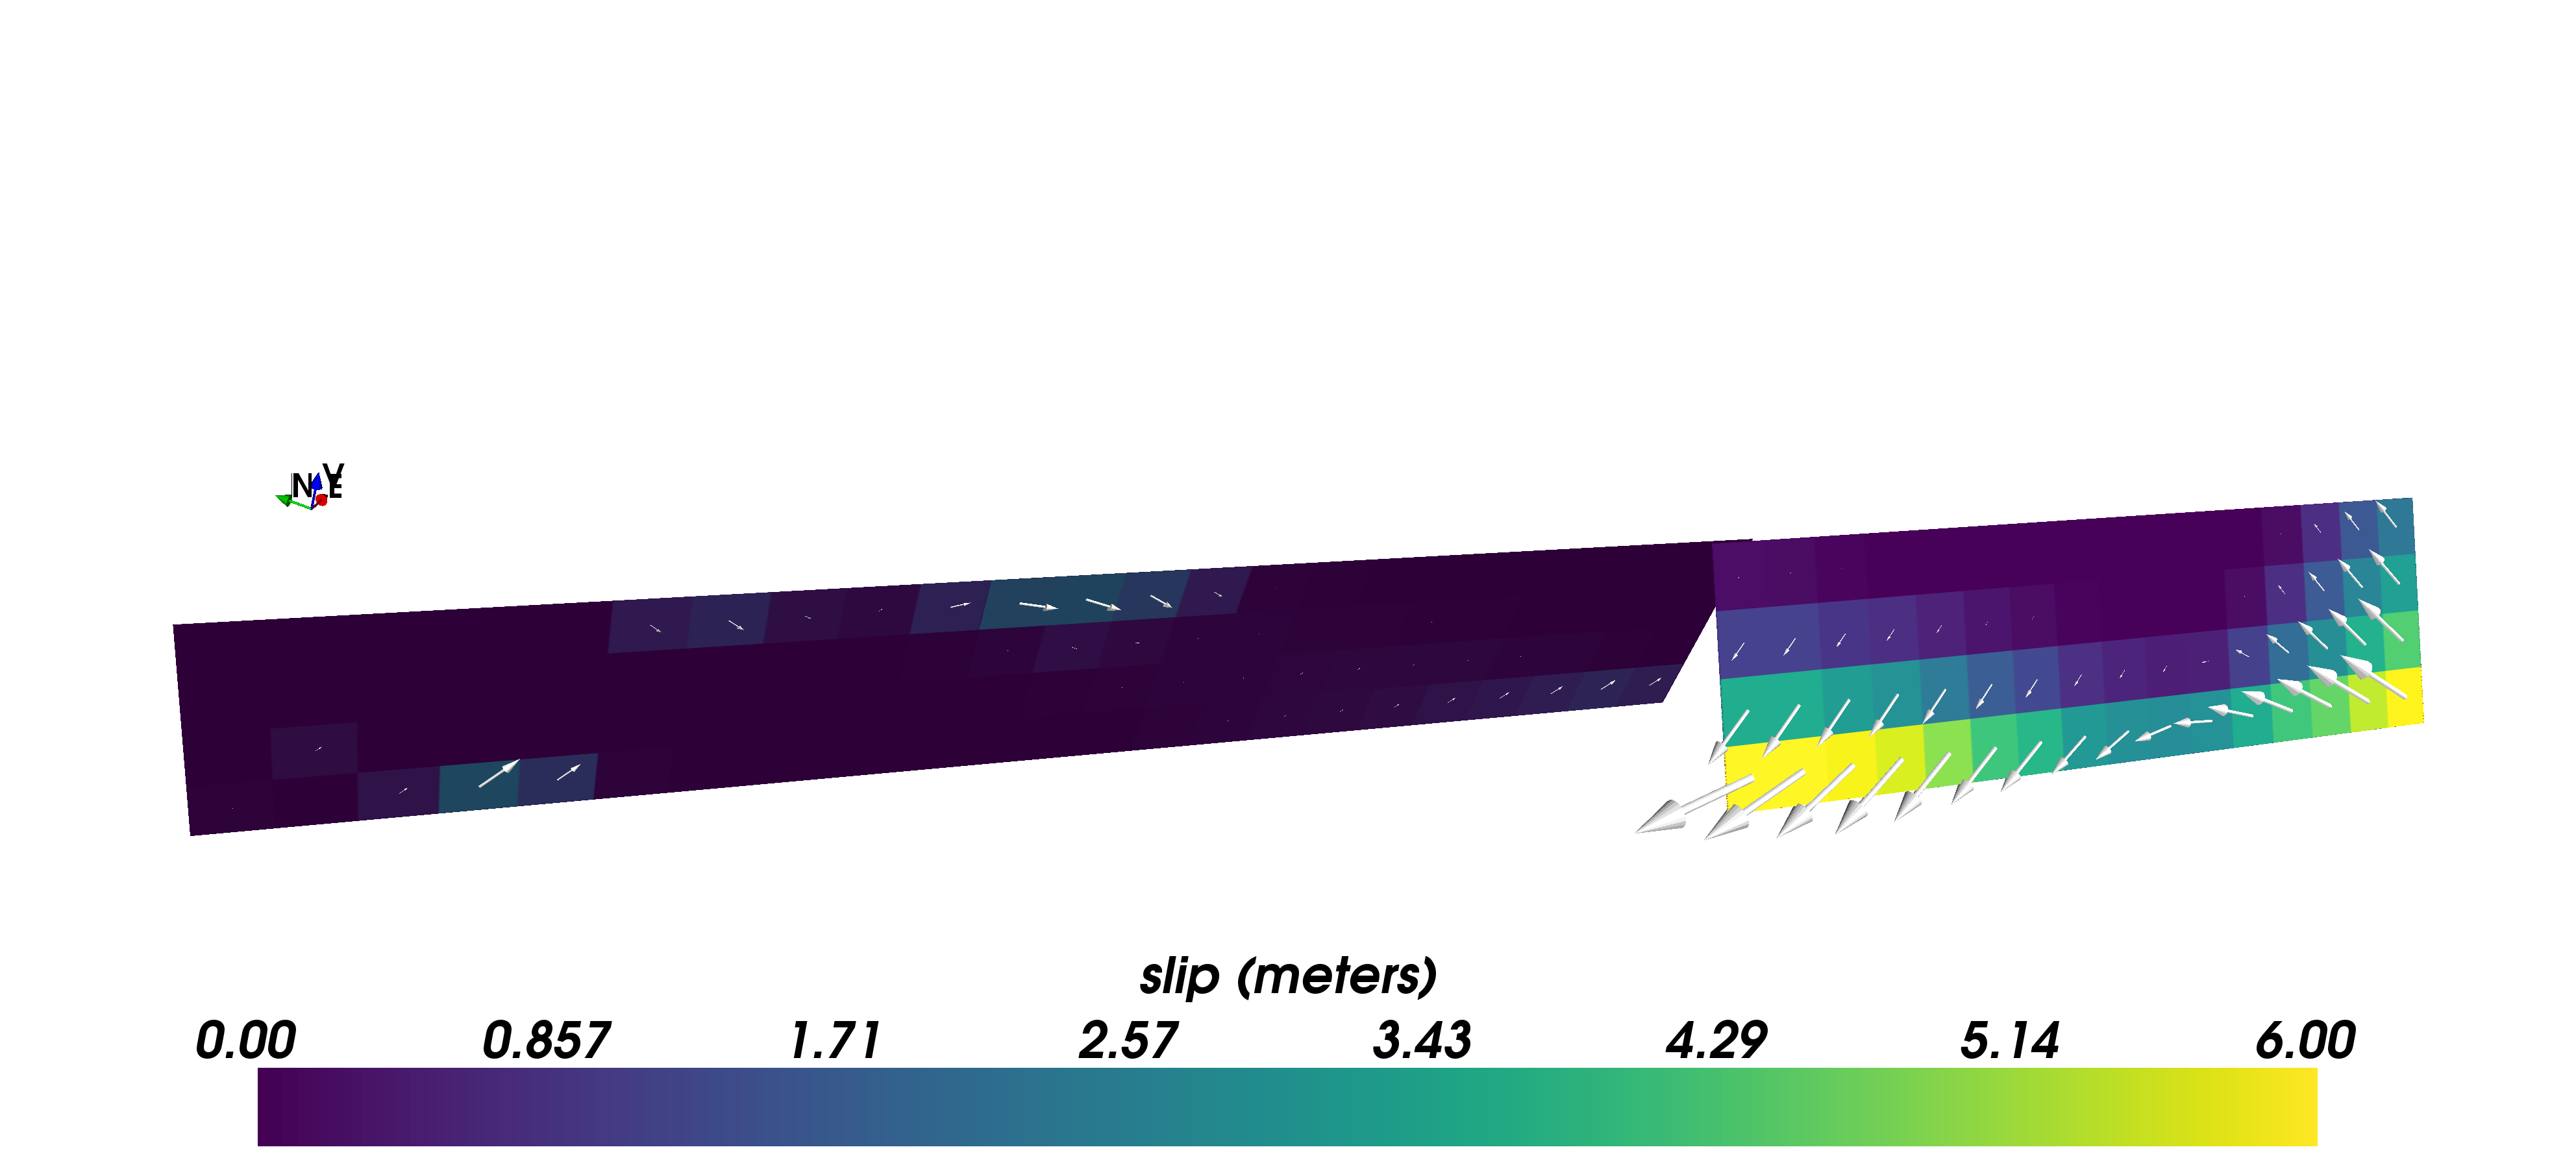
\includegraphics[scale=0.1]{Figures/initial_elastic_afterslip}
\centering 
\caption{afterslip from elastic inversion}
\label{FluidityLCurve}
\end{figure} 

\begin{figure}
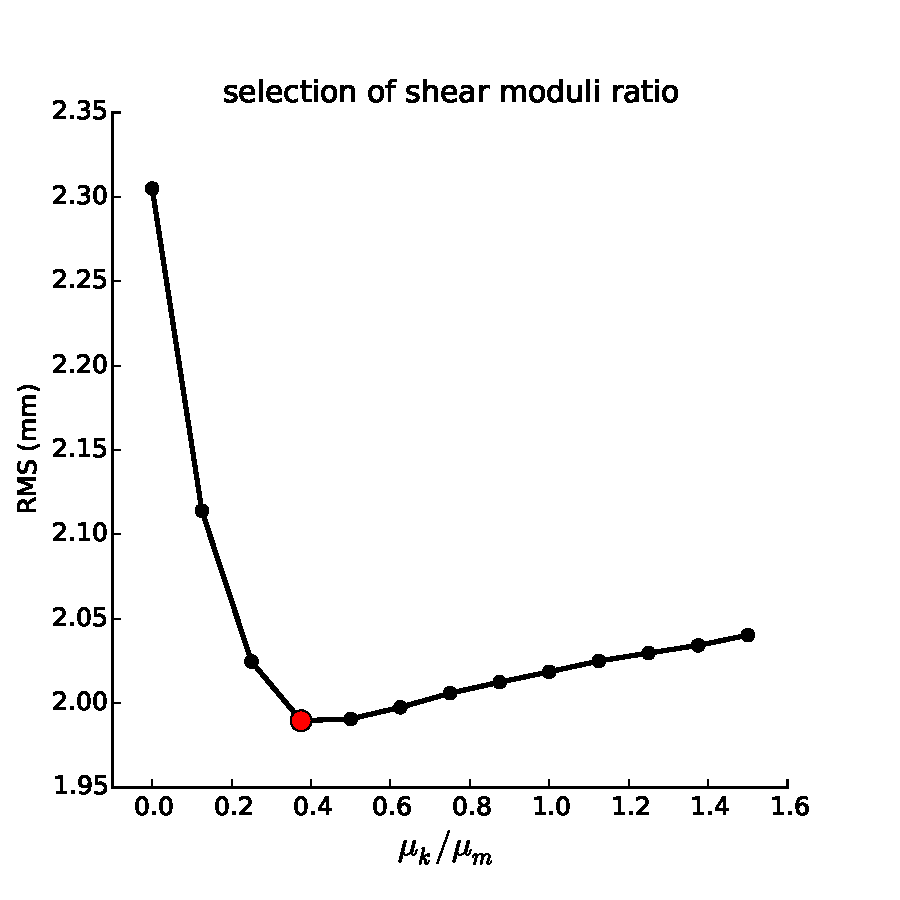
\includegraphics[scale=1.0]{Figures/shear_ratio}
\centering 
\caption{misfit with different shear modulus ratios}
\label{ShearRatio}
\end{figure} 

\begin{figure}
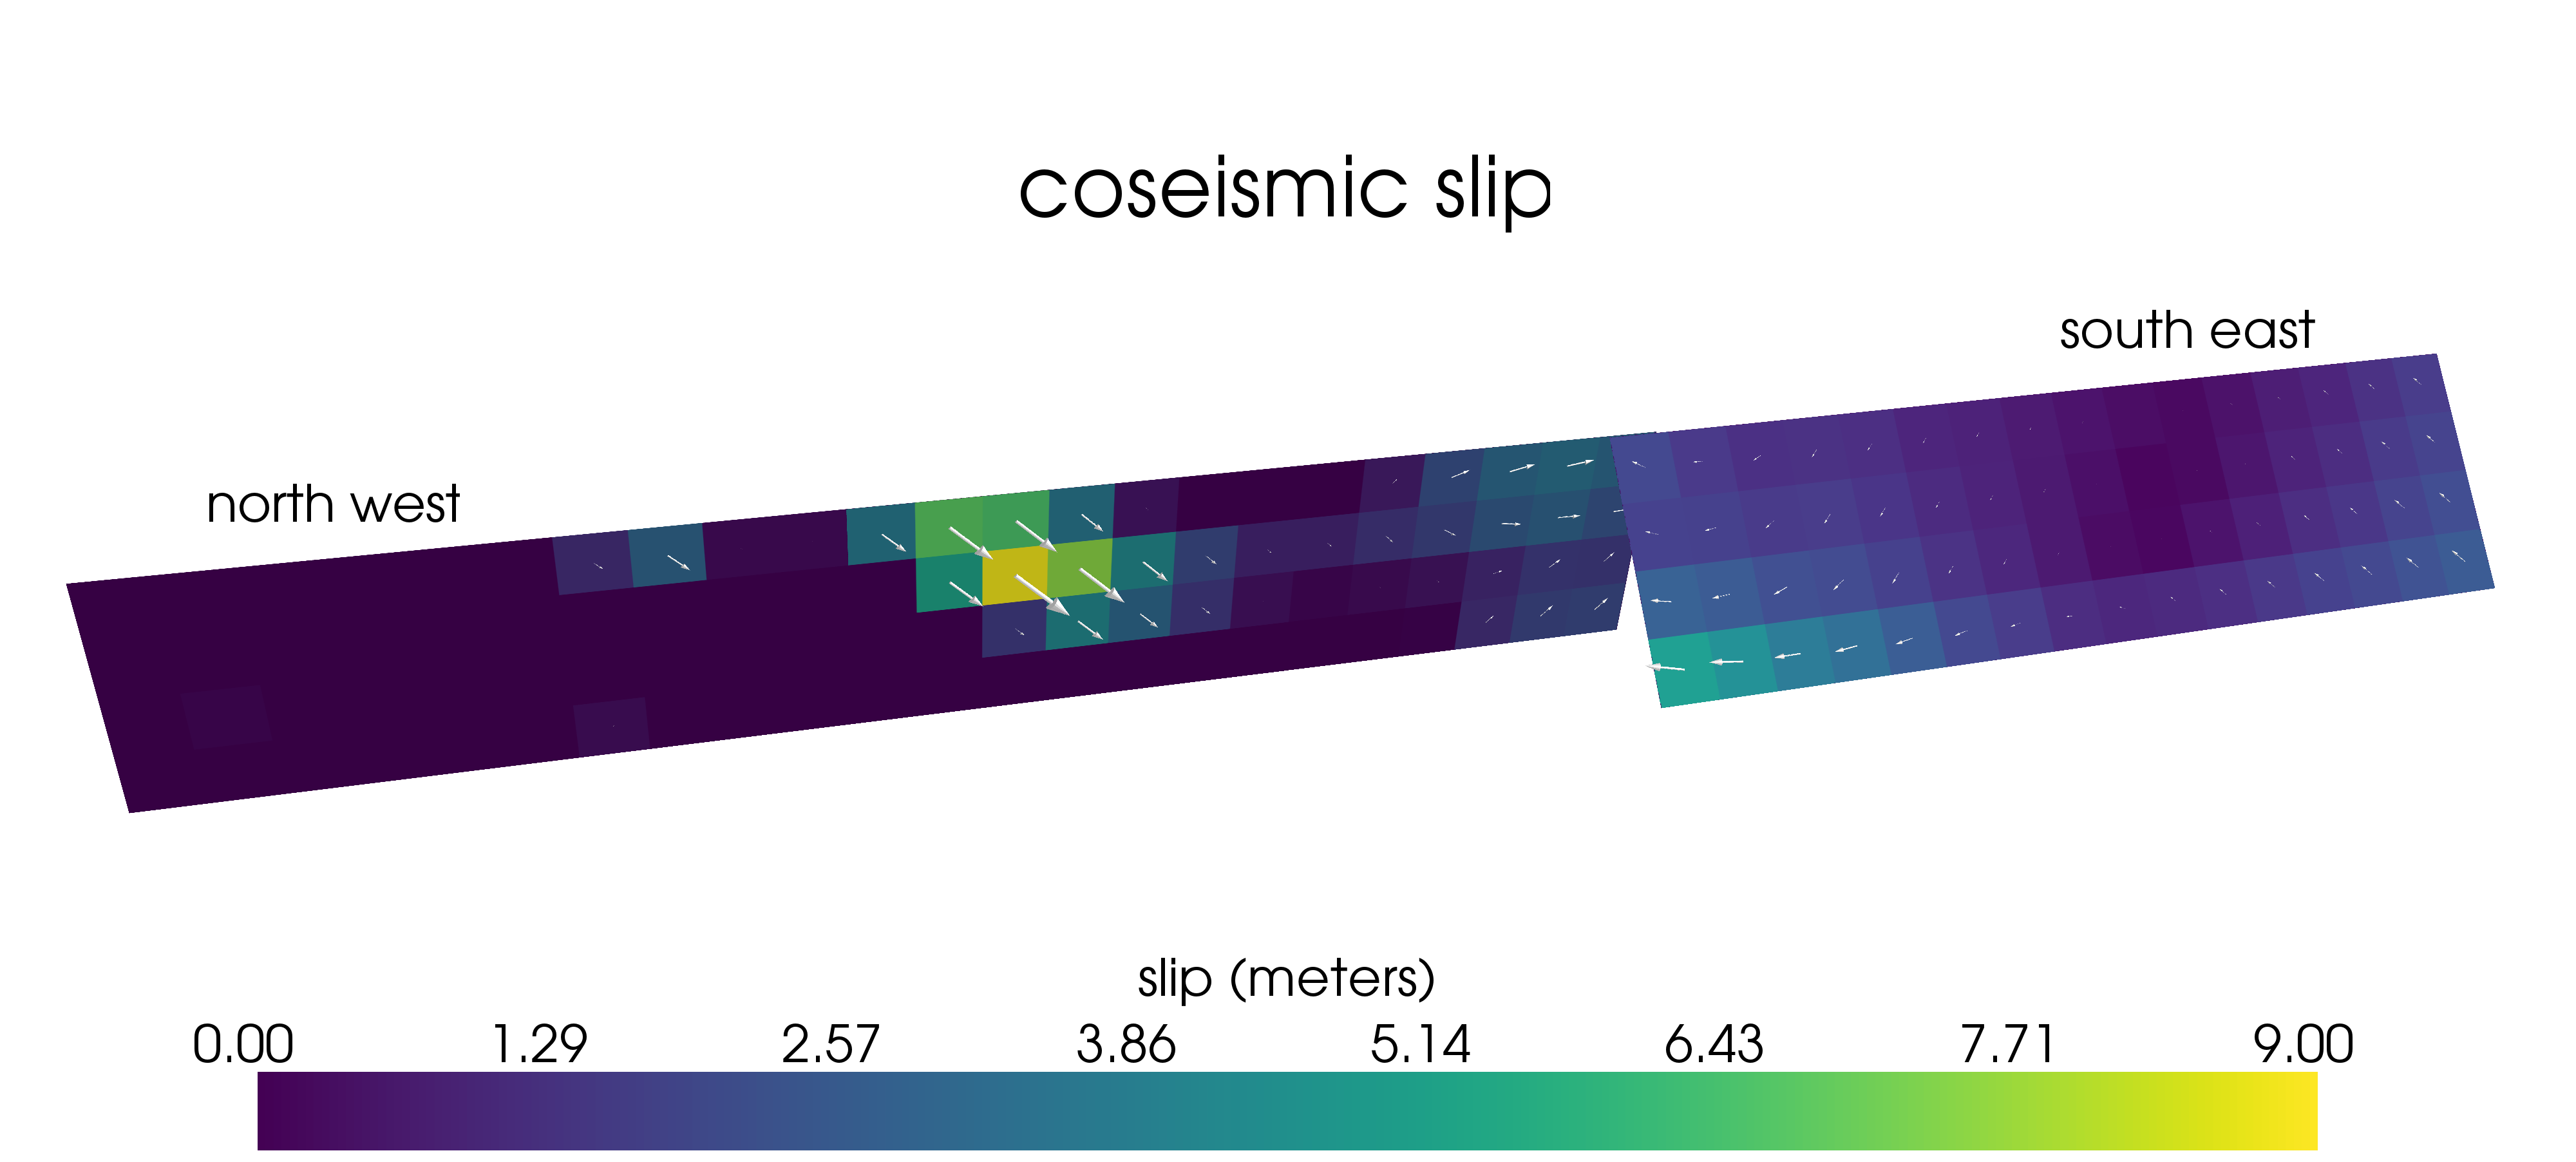
\includegraphics[scale=0.1]{Figures/final_coseismic}
\centering 
\caption{}
\label{FinalCoseismic}
\end{figure} 

\begin{figure}
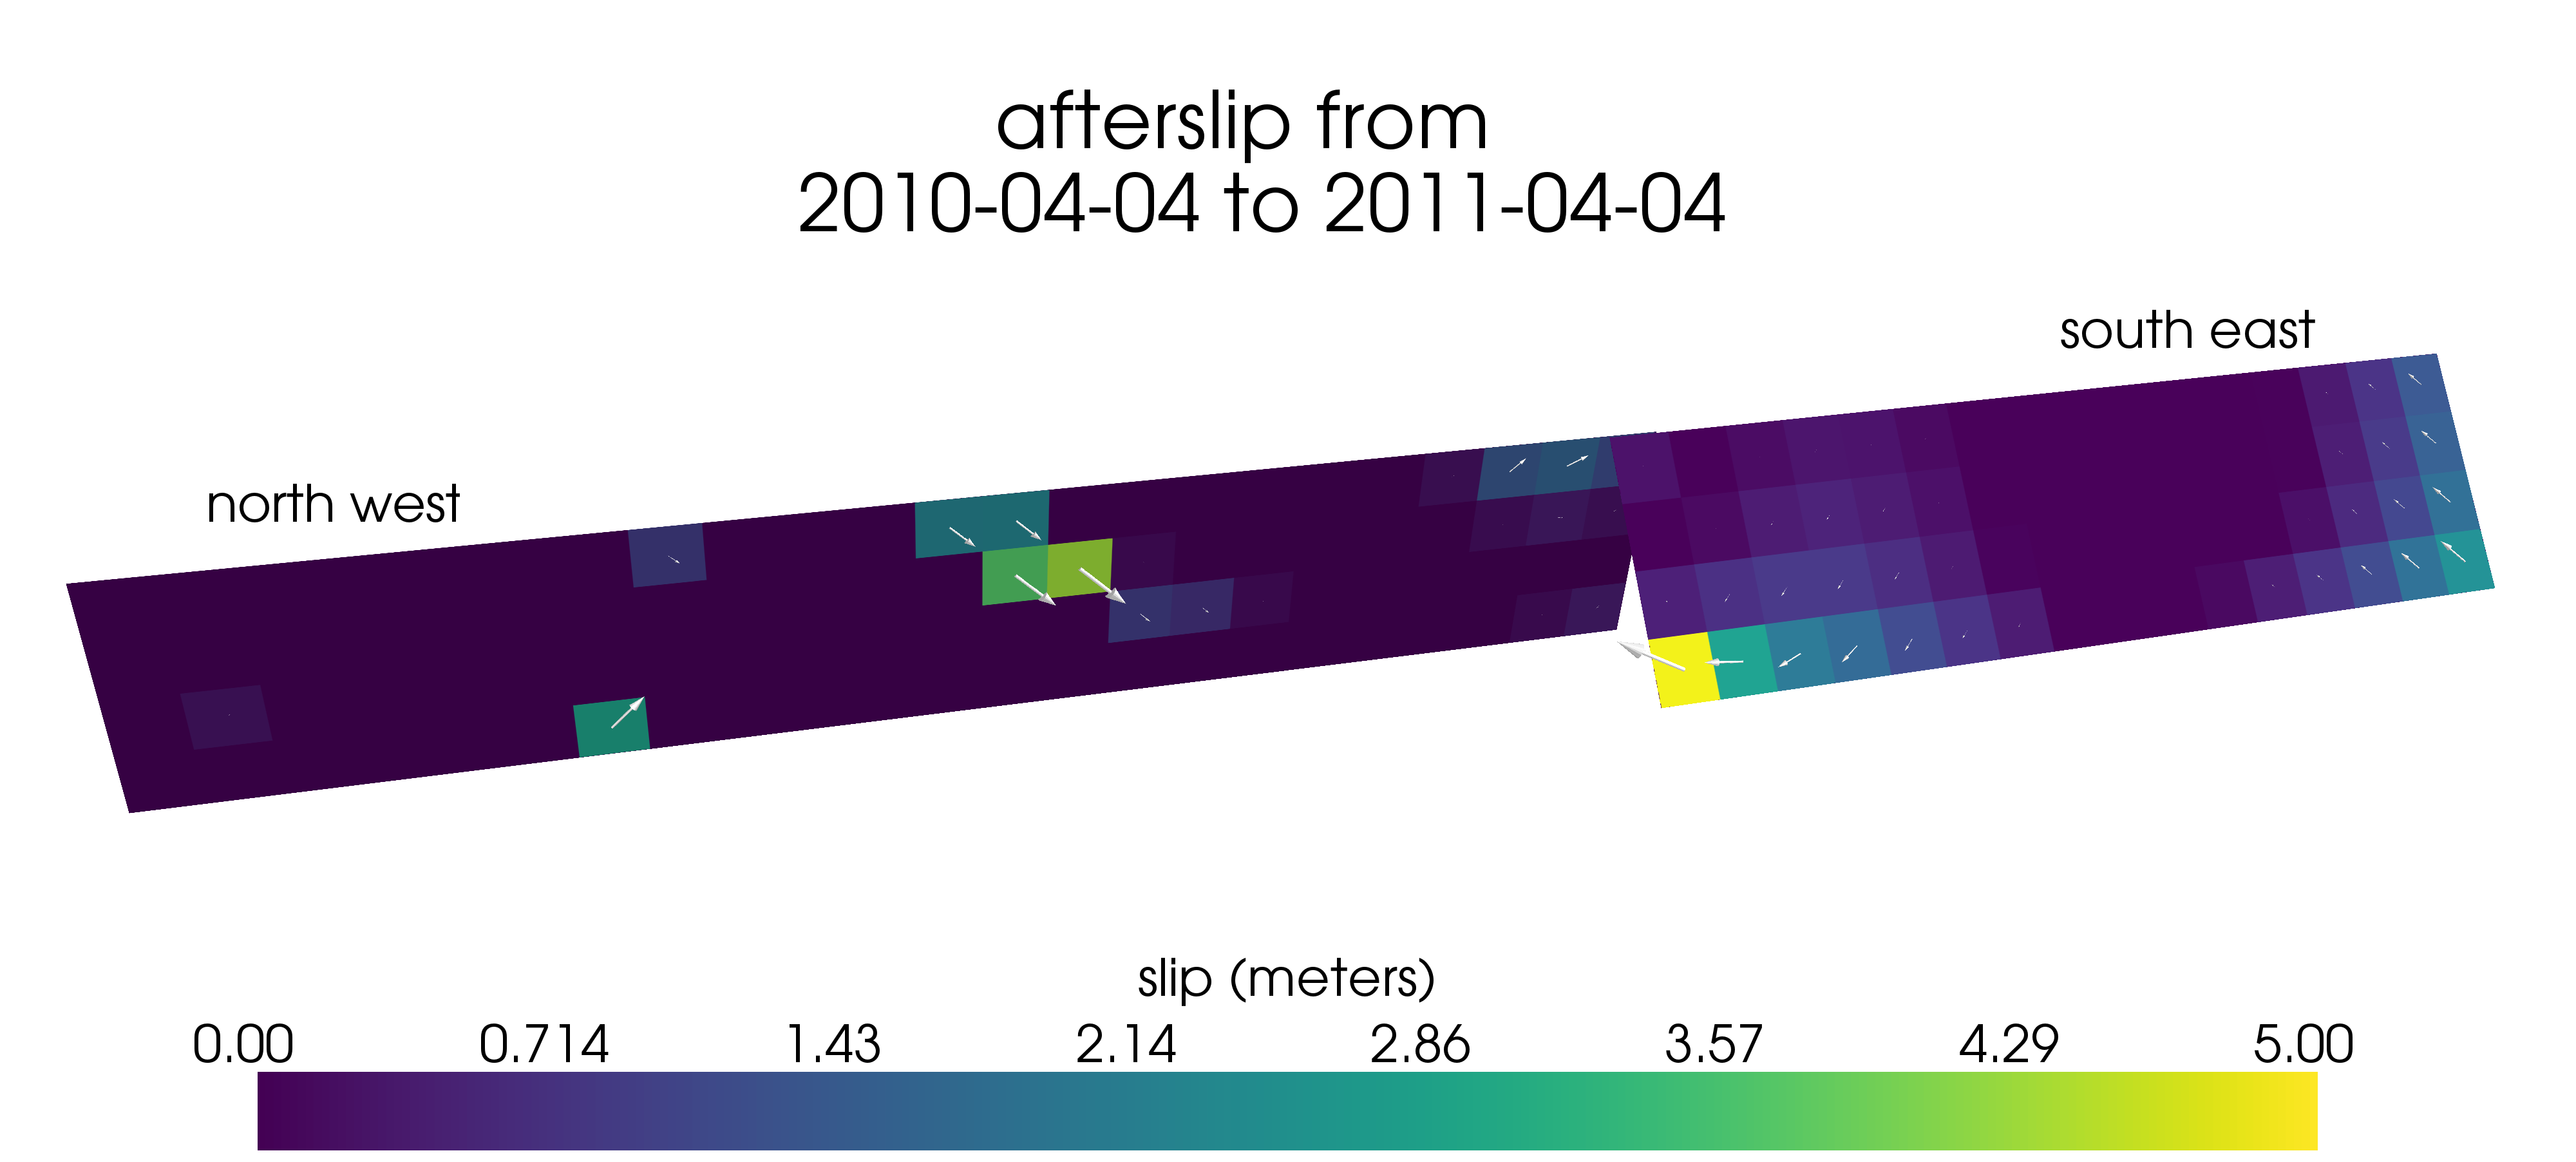
\includegraphics[scale=0.1]{Figures/final_afterslip_0-1}
\centering 
\caption{}
\label{ShearRatio}
\end{figure} 

\begin{figure}
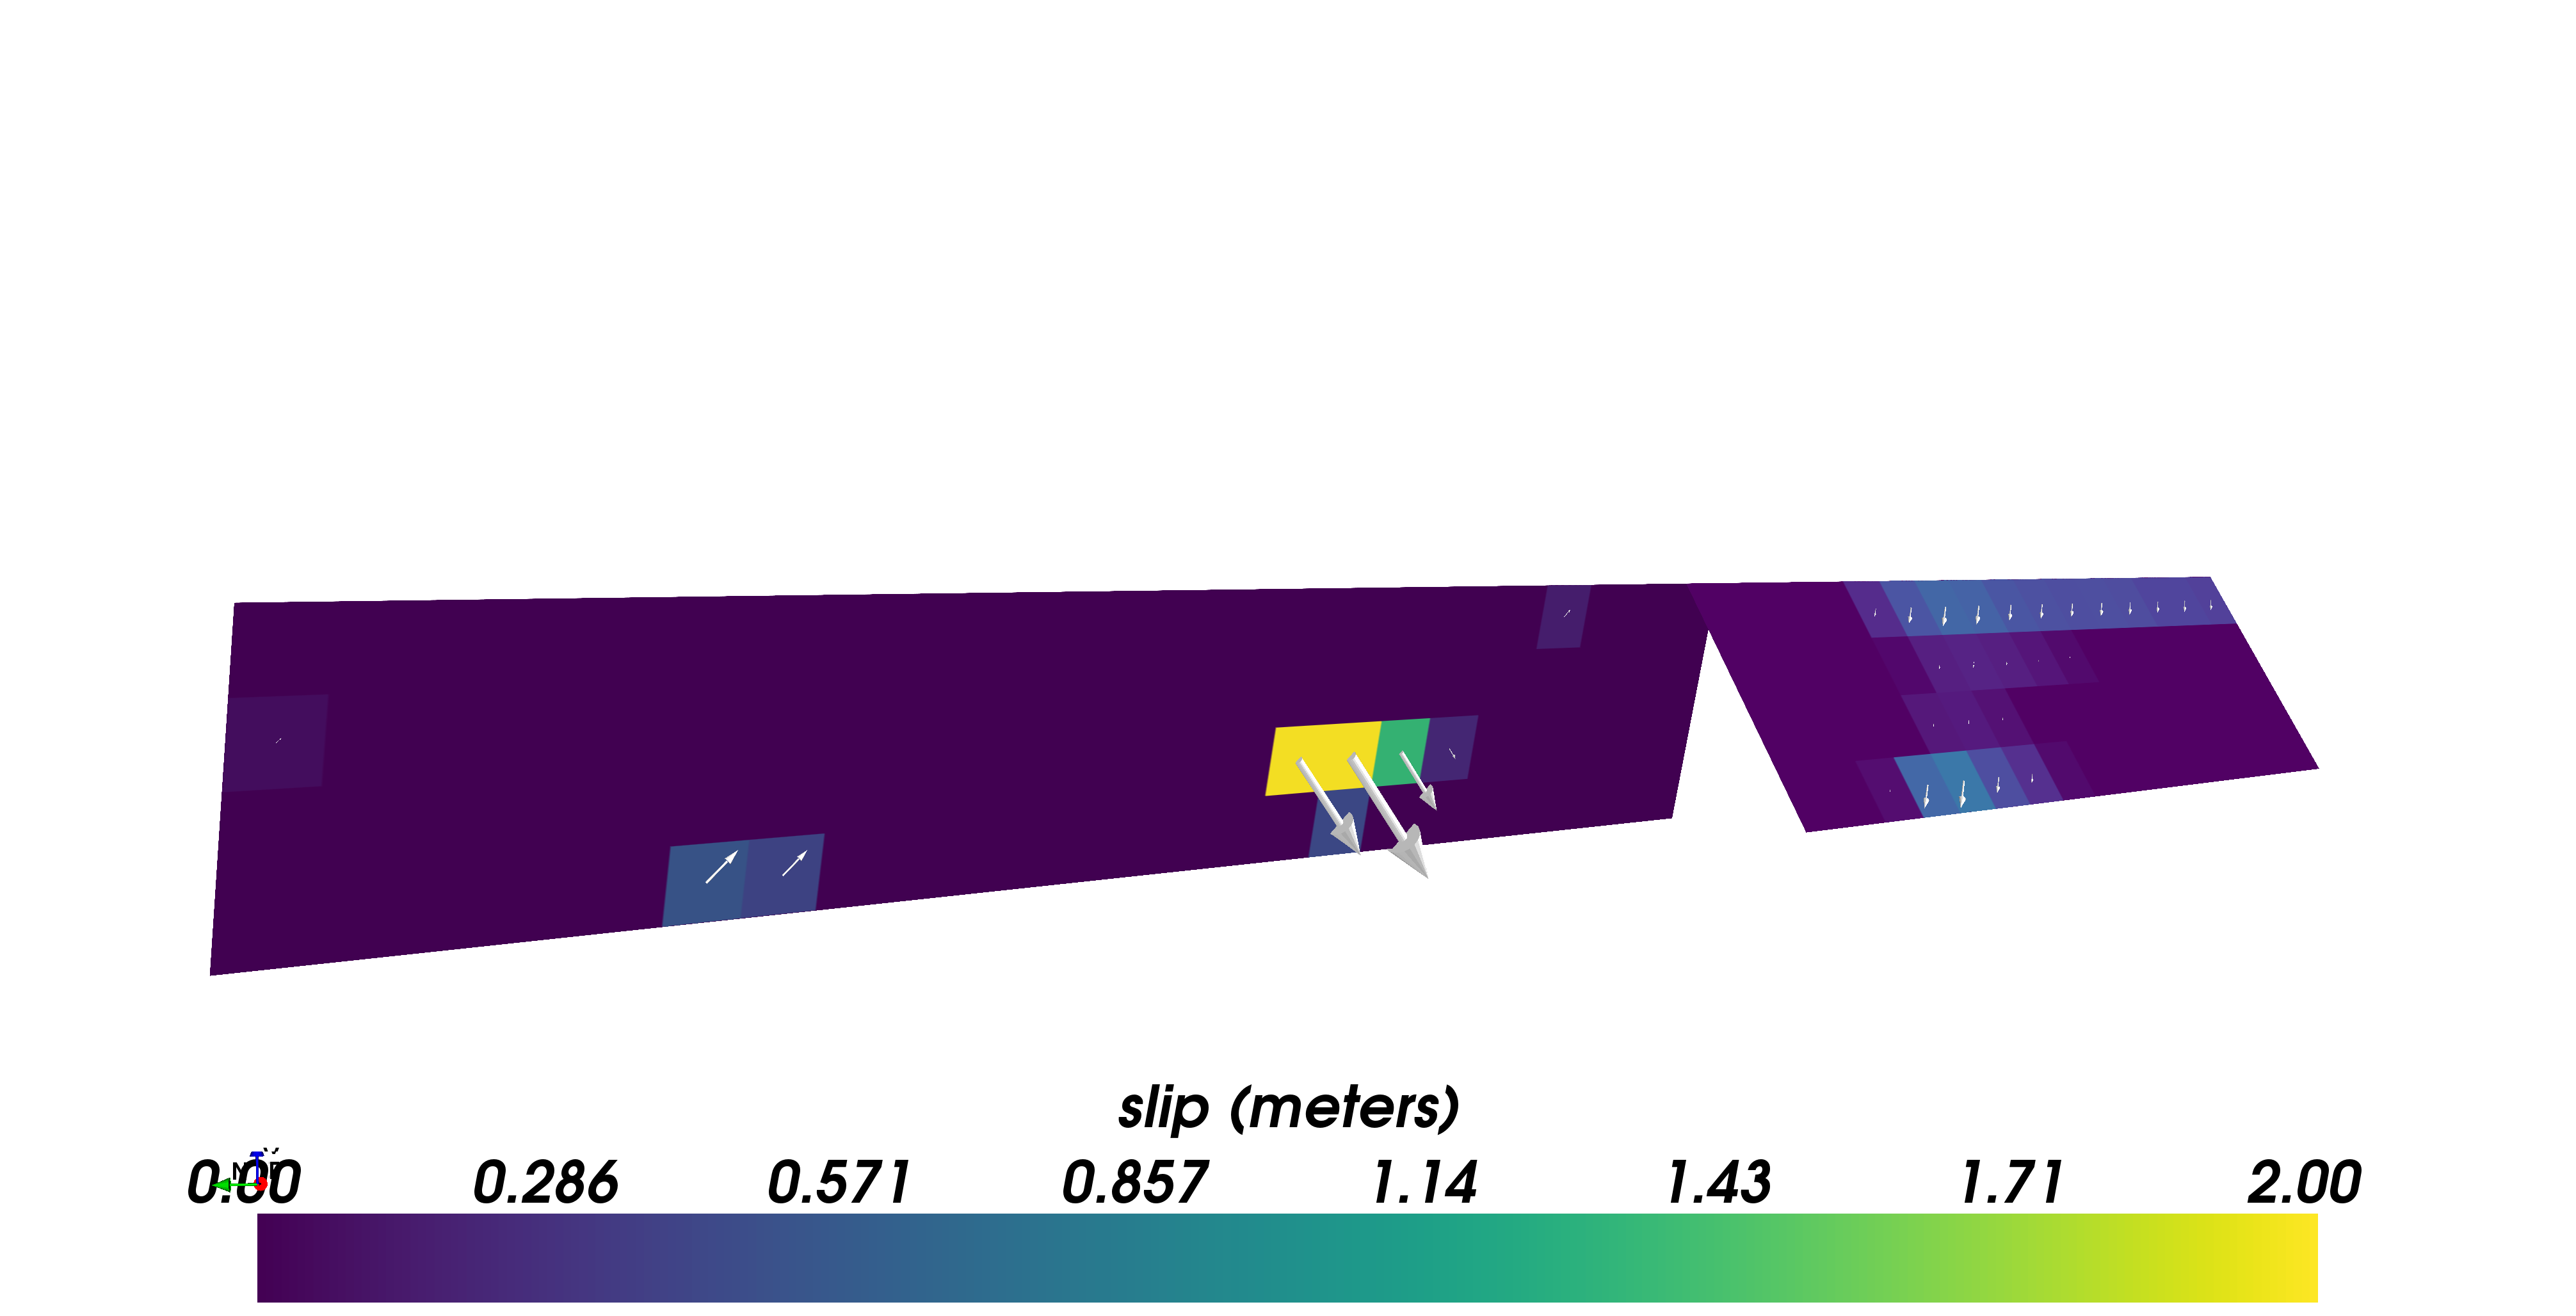
\includegraphics[scale=0.1]{Figures/final_afterslip_1-3}
\centering 
\caption{}
\label{ShearRatio}
\end{figure} 

\begin{figure}
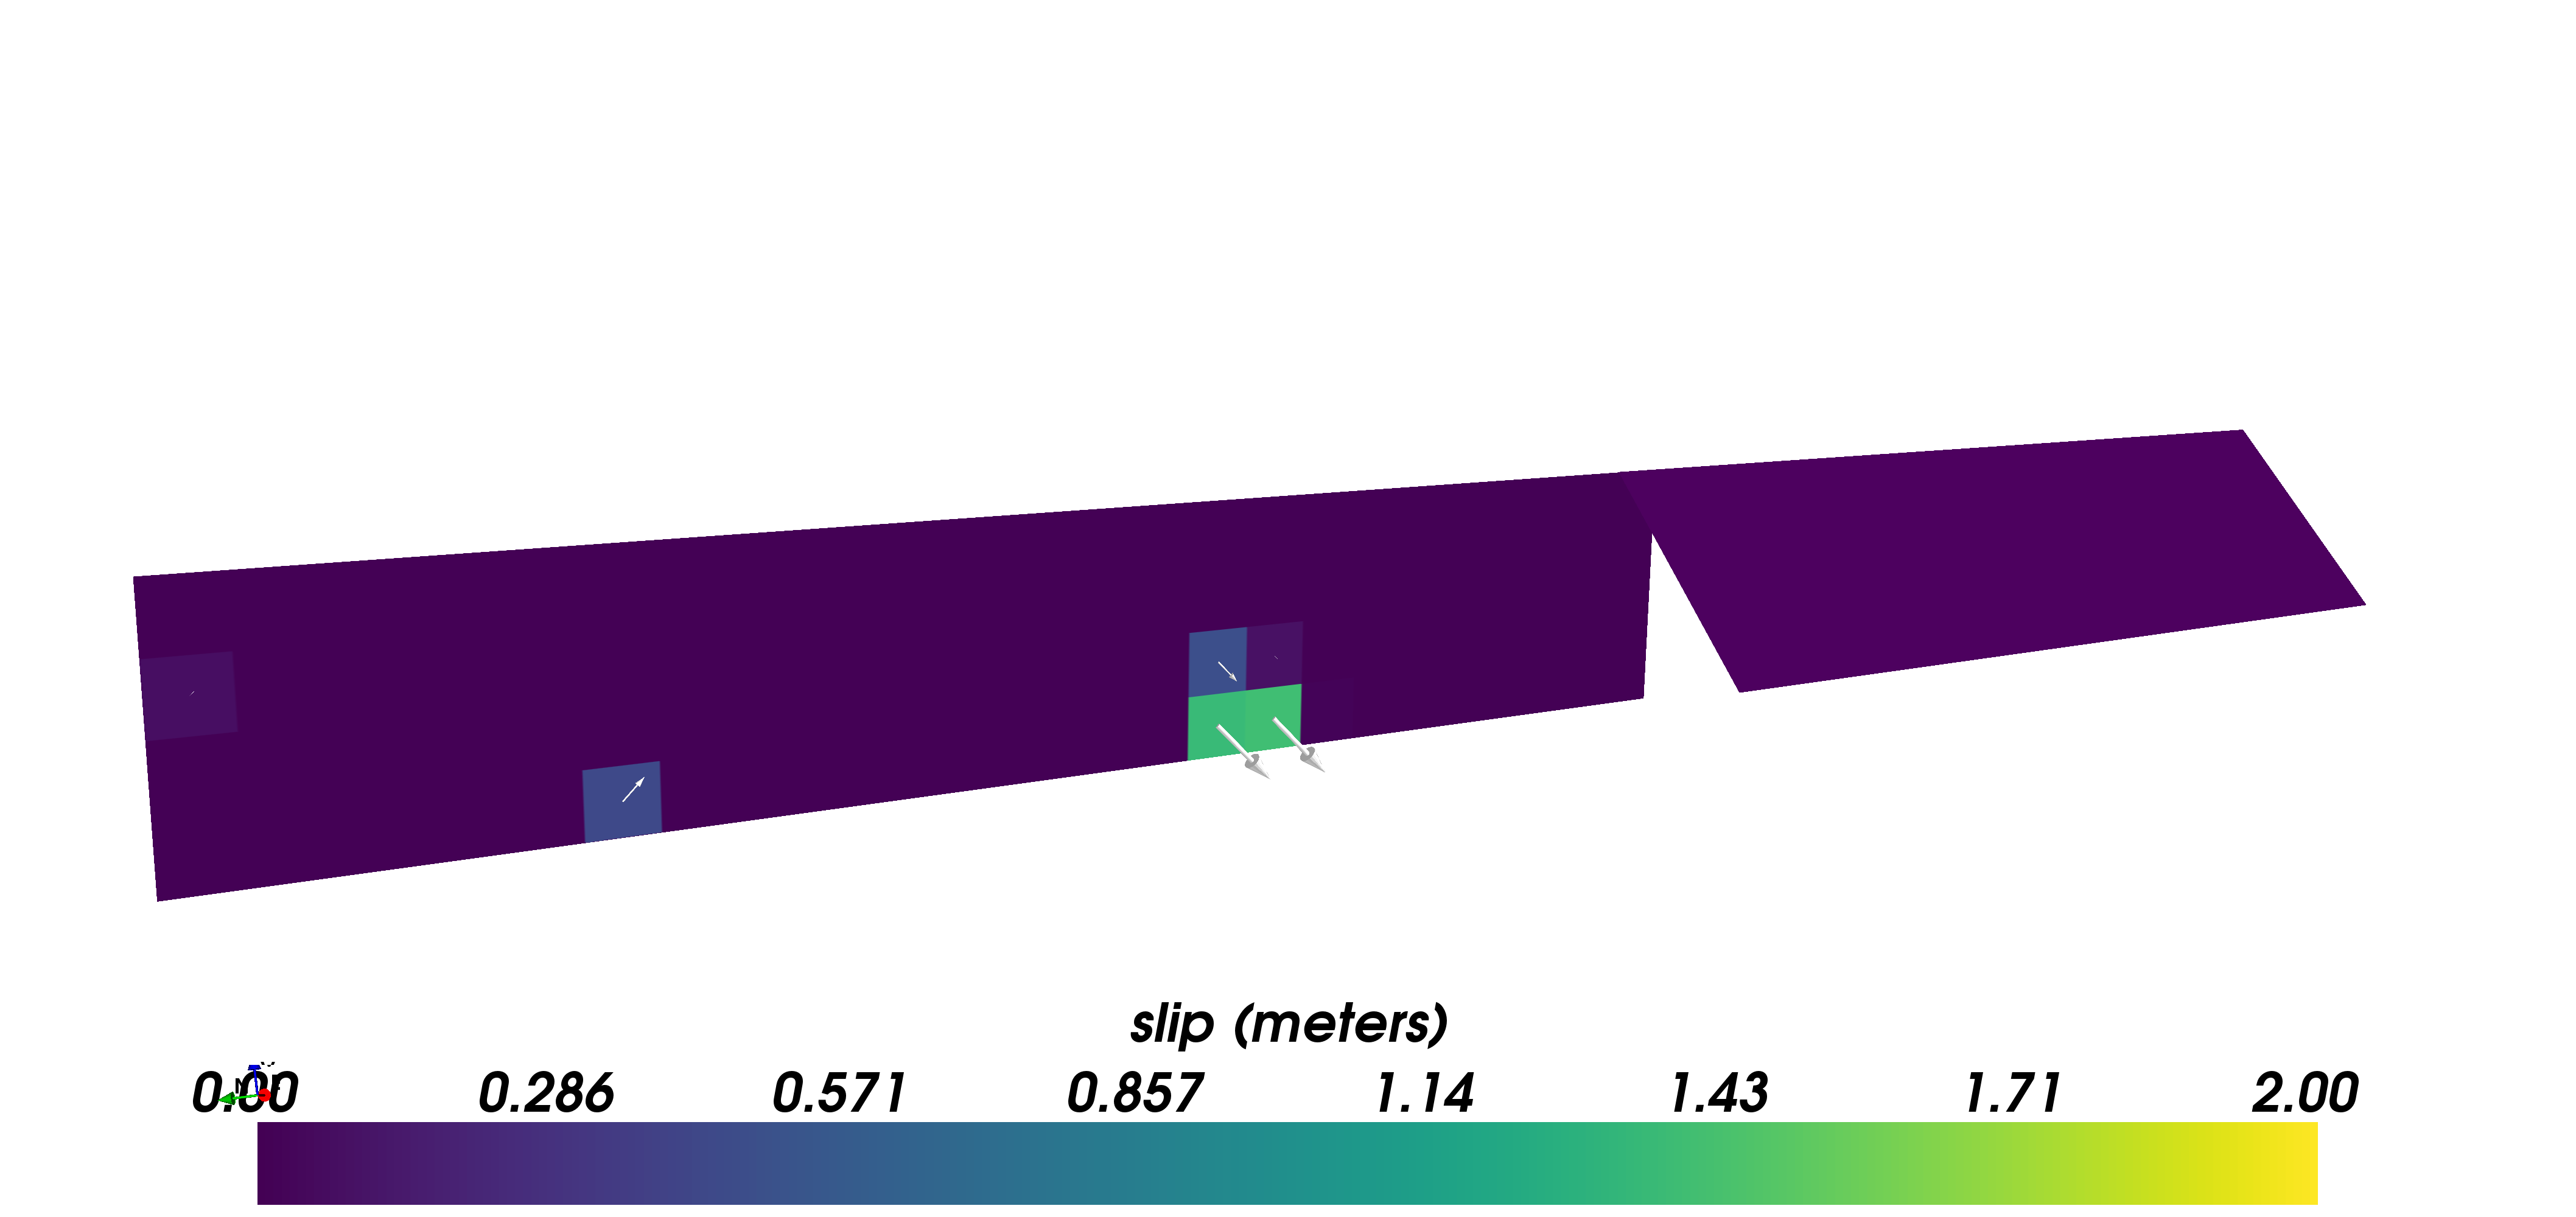
\includegraphics[scale=0.1]{Figures/final_afterslip_3-5}
\centering 
\caption{}
\label{ShearRatio}
\end{figure} 

\begin{figure}
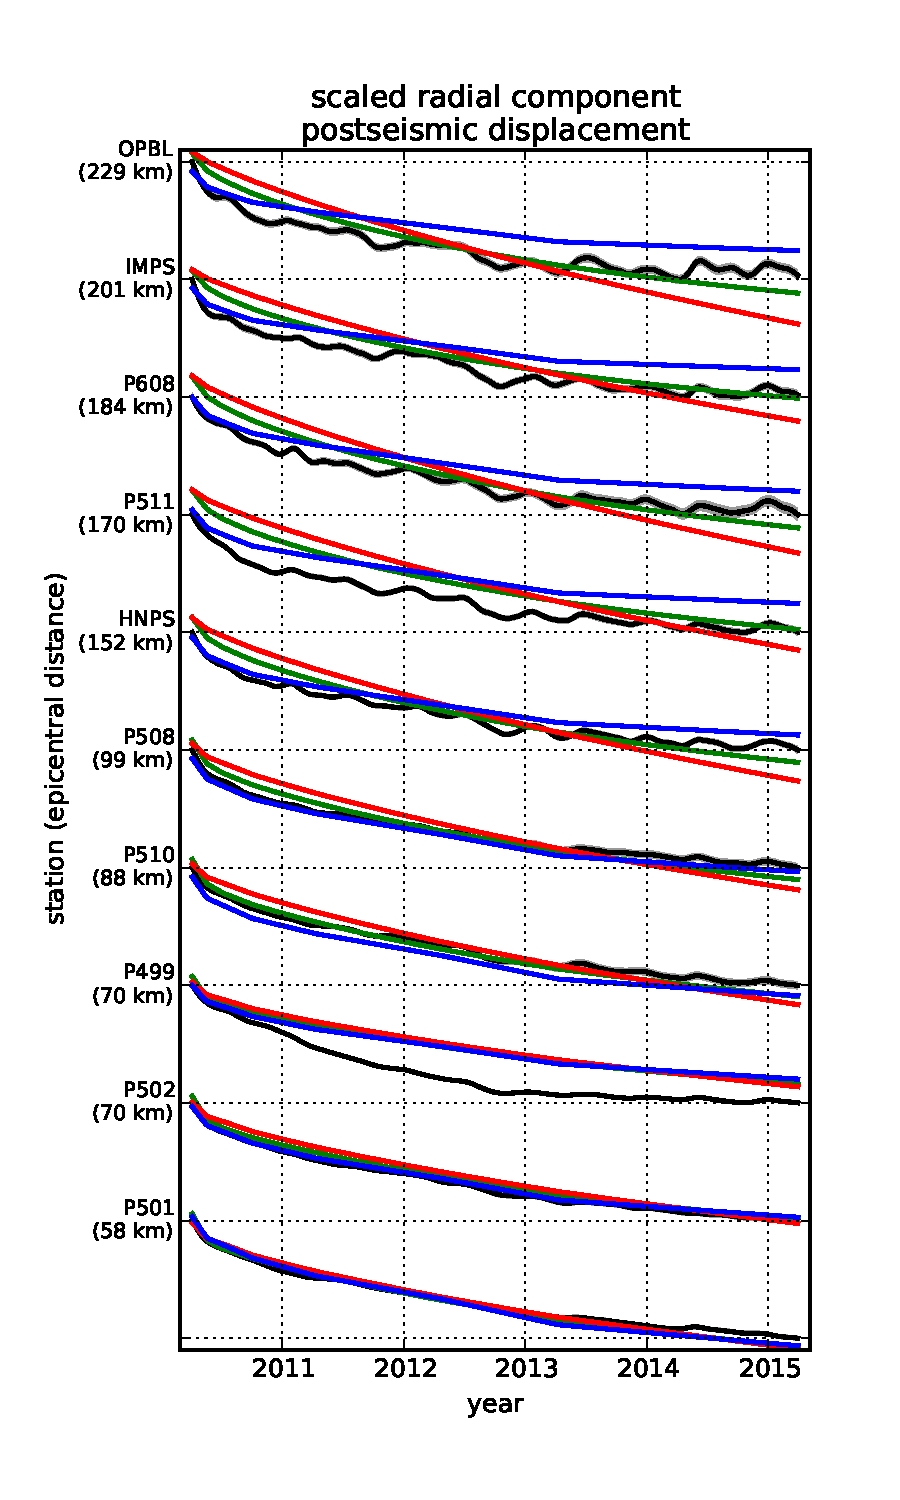
\includegraphics[scale=0.9]{Figures/near_field_final_record_section}
\centering 
\caption{}
\label{ShearRatio}
\end{figure} 

\begin{figure}
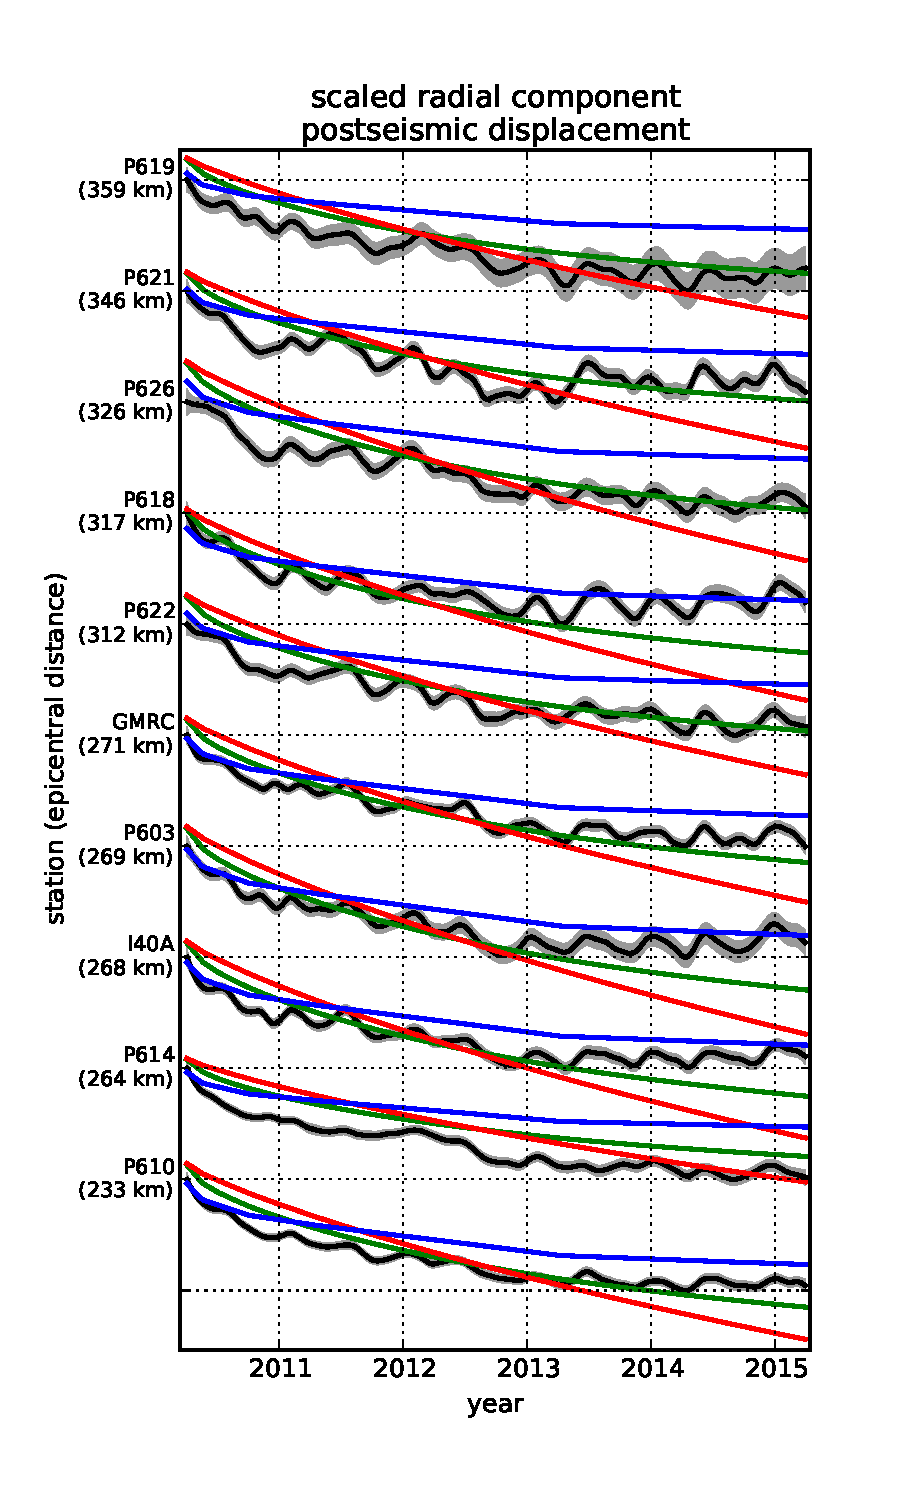
\includegraphics[scale=0.9]{Figures/far_field_final_record_section}
\centering 
\caption{}
\label{ShearRatio}
\end{figure} 



\end{document}

